\documentclass[10pt,a4paper]{article}
\usepackage[utf8]{inputenc}
\usepackage[T1]{fontenc}
\usepackage[margin=2.4cm]{geometry}
\usepackage{booktabs}
\usepackage{tabularx}
\usepackage{graphicx}
\usepackage{amsmath}
\usepackage{xcolor}
\usepackage{url}
\usepackage[hidelinks]{hyperref}
\usepackage{caption}
\usepackage{enumitem}
\captionsetup{font=small,labelfont=bf}
\graphicspath{{../../paper/}}
\setlist{itemsep=1pt,topsep=3pt}
\newcommand{\fitbox}[1]{\resizebox{\ifdim\width>\linewidth\linewidth\else\width\fi}{!}{#1}}

\title{Can We Show That Commercial Language Models Were Trained on a Newspaper's Archive?\\
\large Technical Report: Full Experimental Record (\emph{La Vanguardia})}
\author{Ruben Tous\\ \small Universitat Polit\`ecnica de Catalunya}
\date{\small Technical report accompanying the summary paper (\texttt{paper/paper.tex}) --- \today\\
Status of every experiment: \texttt{docs/experiment\_status.md}}

\begin{document}
\maketitle

\begin{abstract}
We study whether it is feasible to produce evidence, intelligible to a court, that articles from the Spanish
newspaper \emph{La Vanguardia} were used to train commercial large language models (LLMs). We first establish the
provenance facts. The newspaper's full article text is present in Common Crawl, the web corpus underlying most LLM
pre-training sets. The pages also survive standard filtering into ready-made training datasets: the FineWeb-2
dataset holds about 18,000 of them in Catalan and about 310,000 in Spanish, including 82\% of our 2020--2023 test
articles. The site's \texttt{robots.txt} did not exclude AI crawlers from news content until
17 March 2026. We then build a dataset of 1,143 signed, non-agency articles split by publication date into
\emph{members} (2020--2023, before the training-data cutoff of the evaluated models) and \emph{controls}
(September 2025--March 2026, after it). On it we apply four families of tests.
\begin{itemize}
\item \emph{Black-box tests} (verbatim continuation, DE-COP multiple choice and a pairwise variant), on three Claude 4.5
models and on Gemini 3.1 Flash-Lite, show no difference between members and controls.
\item A \emph{targeted sample} of 212 interviews from \emph{La Contra}, a widely reposted series chosen as the content
most likely to be memorized, is not reproduced verbatim by any of five Claude models, including the current Opus~5.5
and Sonnet~5.5. The longest match is 6--8 generic words.
\item \emph{Token-probability tests} on an open-weight commercial model (Qwen2.5-7B) show a weak signal
(AUC $=0.56$, $p<10^{-3}$). It shrinks to AUC $\approx0.53$ once calibrated against a model trained on 2018 data.
\item \emph{Dataset inference}, which tests the collection as a whole, flags all four open-weight models tested
(Qwen2.5, Llama-3.1, Mistral, Gemma-2). It also flags a 2018 model that cannot have seen the articles ($p=0.007$),
so date-based controls alone create false positives. With groups matched by section and length, only Gemma-2 stays
significant ($p=0.009$), and a \emph{neighbour test} shows that this reflects knowledge of the period's events, not
of the newspaper's wording: no model prefers the original text over same-facts rewrites more for members than for
controls. A comparison of two versions of Llama with different cutoffs (same articles, so time effects cancel) shows
the pattern training predicts ($p=0.007$), but it is small and is also explained by knowledge of the events. A
version restricted to wording (original text vs same-facts rewrites) points the same way but is not significant
($p\approx0.07$). A pre-registered replication on new articles points the same way with the same size but is again
not significant ($p=0.097$ and $0.067$), so the effect is not confirmed.
\item A \emph{retrieval test} on the Gemini API shows no answer-time reuse, because its URL tool could not fetch the
site's pages. Without access, the model sometimes invented ``literal'' paragraphs and attributed them to the
newspaper.
\item A cheap \emph{screening test} asks for details that exist (almost) only on the newspaper's website: article
URLs, bylines, interview headings and masked names or figures. No model gives exact answers above the control rate. However,
given only an article's title and date, Gemini 3.1 Flash-Lite predicts the newspaper's internal article number to
within a median of 3 days of the right one for 2021--2023 articles, and fails completely for later ones
($p=3\times10^{-14}$). The model has thus seen many \emph{La Vanguardia} URLs from that period. This flags it for
further tests but does not show memorization of any article.
\end{itemize}
We also report two methodological pitfalls in recognition tests that inflate apparent evidence. We conclude that neither randomly sampled
articles nor the newspaper's most-copied interviews are memorized strongly enough to give per-article evidence with
defensible prompts. The most promising route is dataset inference over thousands of archive articles with same-period
controls (articles never captured by web crawlers), on models whose word probabilities are accessible. Other routes
are retrieval-time use by web-enabled assistants and copyright traps for future content.
\end{abstract}

%======================================================================
\section*{Summary of premises}
The analysis rests on the following premises, stated in plain language. Sections~\ref{sec:legal}--\ref{sec:stats}
give the details and sources.

\paragraph{Legal premises (EU and Spain).}
\begin{itemize}
\item By default, EU law allows copying publicly available text to train AI. This is the ``text and data mining''
(TDM) exception. It has two conditions: the copier must have had \emph{lawful access} to the text, and the owner must
not have reserved its rights.
\item For content published online, the reservation (``opt-out'') must be \emph{machine-readable}. A German appeal
court held in 2025 that a plain-language clause in the terms of use was not enough, at least for 2021.
\item \emph{La Vanguardia} did not opt its news articles out of AI crawlers until \textbf{17 March 2026}. Before that,
only its film and book sections were excluded.
\item A Munich court ruled in November 2025 (\emph{GEMA v.\ OpenAI}) that a model that has \emph{memorized} a work
contains a copy of it, and that the TDM exception does not cover this. The decision is at first instance and is under
appeal.
\item Even today, \texttt{robots.txt} blocks only crawlers that collect \emph{training} data (GPTBot, ClaudeBot,
CCBot, Bytespider). It does not block the agents that fetch pages \emph{at answer time} for AI assistants
(OAI-SearchBot, ChatGPT-User, PerplexityBot) or Google's AI opt-out token (Google-Extended).
\item Therefore, for pre-2026 content, proving that articles were \emph{crawled} is weak. Proving that a model
\emph{memorized} or \emph{reproduces} them is strong.
\item Copies taken from illegal sources (pirate mirrors, paywall-bypass sites) do not meet the ``lawful access''
condition, so the exception does not apply to them.
\item Use of articles \emph{at answer time} (an assistant that searches the web and reproduces an article) is a
different act from training. It may also engage the press publishers' right.
\item Evidence must be obtained lawfully, without bypassing paywalls, and the tests must be simple, fixed in advance
and fully logged. In the \emph{New York Times} case, OpenAI attacked the evidence as ``hacking''.
\end{itemize}

\paragraph{Technical premises.}
\begin{itemize}
\item A language model does not store documents; it learns statistical patterns. It reproduces a text word for word
only if it has seen that text \emph{many times} during training. Song lyrics are copied thousands of times on the
web; a typical news article is not.
\item The articles are not only in raw Common Crawl. They survive the standard quality filters and are inside
ready-made, publicly distributed training datasets. The FineWeb-2 dataset contains about 18,000
\texttt{lavanguardia.com} documents in its Catalan part and about 310,000 in its Spanish part, including 82\% of the
2020--2023 articles we test (Section~\ref{sec:presence}).
\item Knowing the \emph{facts} of an article proves nothing, because facts appear in many sources. Only the
\emph{wording} can identify the source.
\item Every test needs a comparison group: texts the model \emph{could not} have seen, because they were published
after its training data was collected. Without it, a high score can be an artifact.
\item Texts written at different times differ in topics and vocabulary. Part of any difference between old and new
articles is due to time, not to training, and must be subtracted.
\item Most commercial models do not reveal the probabilities they assign to words, which are the most sensitive
signal. With them we can only use ``black-box'' tests (asking questions and reading answers). Full access exists only
for \emph{open-weight} models, whose parameters are published and can be run locally: for example Meta's Llama,
Alibaba's Qwen, Mistral's open models, DeepSeek and Google's Gemma. Among hosted APIs, OpenAI has offered word
probabilities for some non-reasoning models (e.g.\ GPT-4o, GPT-4.1), but only for the words the model generates, not
for a text supplied by the user. The Claude API does not offer them, and none of the Gemini models available to us did
(Section~\ref{sec:setup}).
\item A signal too weak to show for one article can become statistically clear when thousands of articles are
combined.
\item \emph{Copyright traps}, which are unique invented phrases planted in future articles, make later detection far
more reliable. They only work for content published after they are introduced.
\end{itemize}

%======================================================================
\section{Introduction}
Several lawsuits by publishers and rights holders against AI developers have reached the courts
(Section~\ref{sec:legal}). In most of them a central factual question is whether, and how, protected works were
used to build a model. Developers rarely disclose their training corpora, so plaintiffs must infer use from the
behavior of the deployed model. This study asks a practical question for \emph{La Vanguardia} (Grupo God\'o):
\emph{with publicly available tools and the publisher's own archive, can training use be demonstrated
convincingly enough to present to a judge?}

The intended audience is legal, so we favor tests that are (i)~explainable without machine-learning background,
(ii)~paired with explicit controls, (iii)~reproducible from logged queries, and (iv)~obtained without circumventing
any access control. This report covers the first, exploratory phase. It uses articles obtained from Common Crawl,
because the licensed archive was not yet available, and models reachable at low cost.

\paragraph{Contributions.}
\begin{enumerate}[label=(\arabic*)]
\item A provenance analysis: the newspaper's text is in Common Crawl, and its AI opt-out has a precise date.
\item A reproducible pipeline that collects articles with record-level provenance and logs every model query with a
tamper-evident hash.
\item A pilot comparison of black-box and token-probability tests on seven commercial models, with temporal controls
and a drift-calibrated reference model.
\item Two methodological pitfalls that would otherwise produce false evidence.
\item A feasibility assessment and research plan.
\end{enumerate}

%======================================================================
\section{Legal context}\label{sec:legal}
\emph{This section summarizes public sources for orientation. It is not legal advice and must be validated by
counsel.}

\subsection{Key cases and their outcomes}
Table~\ref{tab:cases} lists the cases most relevant to this study and their status as of November 2026.

\begin{table}[h]\centering\footnotesize
\begin{tabularx}{\linewidth}{>{\raggedright\arraybackslash}p{2.6cm}>{\raggedright\arraybackslash}X>{\raggedright\arraybackslash}X}
\toprule
Case & What was argued / shown & Outcome (status Nov.\ 2026)\\
\midrule
\emph{GEMA v.\ OpenAI}, LG M\"unchen~I, 42~O~14139/24 &
ChatGPT reproduced the lyrics of nine German songs in response to simple prompts. &
\textbf{OpenAI lost at first instance} (11 Nov.\ 2025): injunction, disclosure and damages. Memorization in the model
is a reproduction (\S16 UrhG), and outputs are reproduction and communication to the public. The TDM exception does
not apply. OpenAI appealed in December 2025; the appeal is pending.\\
\emph{NYT v.\ Microsoft \& OpenAI}, S.D.N.Y.\ (MDL 3143) &
About 100 examples of GPT-4 completing NYT articles near-verbatim (``Exhibit J''); also claims on training and on
retrieval (``grounding''). &
\textbf{Pending.} Core claims survived dismissal (2025). Discovery of output logs was ordered (2026). Cross-motions for
summary judgment were filed in September 2026, with no ruling and no trial date yet. See Section~\ref{sec:nyt}.\\
\emph{Bartz v.\ Anthropic}, N.D.~Cal. &
Authors' books used for training, some downloaded from pirate libraries. &
Training held to be \textbf{fair use} (June 2025), but building a library from pirated copies was not. Ended in a
\textbf{\$1.5\,bn class settlement}, approved in July 2026.\\
\emph{Kadrey v.\ Meta}, N.D.~Cal. &
Authors' books used to train Llama. &
\textbf{Meta won summary judgment on fair use} (June 2025), because the plaintiffs showed no market harm. The ruling
was limited to those plaintiffs; a residual claim continued.\\
\emph{Thomson Reuters v.\ Ross}, D.~Del.\ / 3d~Cir. &
Westlaw headnotes used to train a competing (non-generative) legal search tool. &
\textbf{Not fair use}. Affirmed by the Third Circuit on 29 Sept.\ 2026, the first US appellate ruling on AI training.
It is narrow: the tool was not generative.\\
\emph{Getty Images v.\ Stability AI}, UK High Court &
Images used to train Stable Diffusion; Getty watermarks appeared in some outputs. &
\textbf{Getty largely lost} (4 Nov.\ 2025). The model weights do not store copies of the images, so the model is not
an ``infringing copy''. A narrow trademark win on watermarked outputs. Permission to appeal was granted in Dec.\ 2025.\\
\emph{Kneschke v.\ LAION}, LG / OLG Hamburg &
A photo used in a training dataset despite a no-scraping clause in the stock site's terms. &
\textbf{Photographer lost} (2024; appeal dismissed 10 Dec.\ 2025). The dataset was covered by the research TDM
exception. The OLG held that a natural-language clause was not ``machine-readable'' (for 2021). A further appeal to
the BGH was allowed.\\
\emph{Folha de S.Paulo v.\ OpenAI} (Brazil) & Newspaper content used by ChatGPT. & Reportedly ended in a licensing
agreement.\\
\bottomrule
\end{tabularx}
\caption{Relevant cases. The pattern is that courts have been receptive when a model demonstrably
\emph{reproduces} protected text (GEMA), and skeptical when only training on the work is shown and the model does not
contain copies (Getty, Kadrey). In the US, how the copies were \emph{obtained} has mattered (Bartz).}
\label{tab:cases}
\end{table}

\subsection{The \emph{New York Times} ``hacking'' dispute}\label{sec:nyt}
The NYT case is the clearest example of how regurgitation evidence is attacked, and it shaped our protocol. Exhibit~J
of the complaint (December 2023) showed about one hundred cases in which GPT-4, given the opening of a Times article,
produced long passages of its continuation nearly word for word. These were presented side by side with the
original, with copied text highlighted. That format is easy for a judge to understand.

In its February 2024 motion to dismiss, OpenAI responded that the Times had ``paid someone to hack'' its products.
It claimed the examples required ``tens of thousands of attempts''. It also said the prompts contained long excerpts of
the articles themselves, relied on a bug, and used ``deceptive prompts that blatantly violate OpenAI's terms of use''.
The point of the argument is that the outputs did not reflect how ordinary users interact with ChatGPT, so they
showed neither a realistic harm nor a substitute for the newspaper. The Times answered that what OpenAI called
``hacking'' was simply using OpenAI's products to look for evidence that they had copied its works. The court did not
dismiss the core claims. The question of how often regurgitation \emph{actually} happens moved to discovery. In 2026
the court ordered production of tens of millions of ChatGPT output logs, including logs from before a regurgitation
filter was added. OpenAI has since argued that the publishers lack evidence of \emph{systematic} regurgitation.

Three lessons follow for this project.
\begin{enumerate}[label=(\alph*)]
\item \textbf{Report the denominator.} State how many attempts were made and how many succeeded, not only the
successes. Our logs record every query, including failures.
\item \textbf{Fix prompts in advance and keep them neutral.} We use one short instruction (``continue the following
text'') and a fixed prefix length. We use no jailbreaks and no repeated sampling until success.
\item \textbf{Separate two legal questions.} Adversarial extraction weakens an argument about what ordinary users
receive (the \emph{output} claim). It does not weaken the argument that the model \emph{contains} the work. Under the
\emph{GEMA} reasoning, memorization is itself a reproduction, and the way the text is coaxed out only proves that the
copy exists. Stronger extraction may therefore still be useful for a memorization claim, as long as it is clearly
labeled as such.
\end{enumerate}

\subsection{What is lawful and what is not}\label{sec:lawful}
\paragraph{Training on publicly available articles (EU/Spain).} Article~4 of the DSM Directive (EU)~2019/790, which
Spain transposed in art.~67 of the Intellectual Property Law (TRLPI), allows reproductions for text and data mining
under two conditions: (i)~\emph{lawful access} to the work, and (ii)~no reservation of rights by the rightholder ``in
an appropriate manner, such as machine-readable means'' for content made publicly available online. Article~3 allows
TDM by research organizations for scientific research \emph{without} any opt-out. That is why LAION, a non-profit
dataset builder, won in Hamburg. The AI Act (Art.~53(1)(c)--(d), applicable since August 2025) requires
general-purpose model providers to have a policy for respecting such reservations, and to publish a summary of their
training content. This creates a documentary avenue for litigation.

\paragraph{Timing of the opt-out.} A reservation applies from the moment it is expressed. Copies made earlier under
the exception are arguably lawful. \emph{La Vanguardia}'s full block of AI crawlers dates from 17~March~2026, so
crawling of news articles before that date is arguably covered by Art.~4. Whether the \emph{continued use} of earlier
copies to train new models after March 2026 is covered is debated.

\paragraph{What if the article is obtained from another source?}
\begin{itemize}
\item \emph{Common Crawl and similar corpora.} Common Crawl is a non-profit that publishes web snapshots. Its own
collection may fall under research TDM, but AI companies reuse its copies commercially. The relevant question is
whether the Art.~4 conditions were met when the developer made \emph{its} copy. For \emph{La Vanguardia} before March
2026, CCBot was not blocked, so those snapshots carry no reservation.
\item \emph{Licensed or syndicated copies} (aggregators, partner sites, press-clipping services). Access is lawful,
but the reservation on \texttt{lavanguardia.com} may not be visible on the third-party site. Whether a reservation
``travels with the work'' is unsettled. Syndication contracts should therefore require partners to reproduce the
opt-out.
\item \emph{Unlawful copies} (pirate mirrors, paywall-bypass sites, scraped republications). These fail the
lawful-access condition, so the exception does not apply. The US \emph{Bartz} case also turned on the illegal origin
of copies. Showing that a model reproduces \emph{paywalled} text could thus point to an unlawful acquisition path, but
the inference requires care.
\end{itemize}

\paragraph{Memorization and outputs.} According to \emph{GEMA}, the TDM exception covers copying \emph{in order to}
analyze text, not a model that ends up containing the work. A memorized article is a reproduction in the model, and
outputs that reproduce it are reproductions and communications to the public. Neither is covered by Art.~4. In the UK,
\emph{Getty} reached the opposite factual conclusion for an image model whose weights were found not to store the
images. The decisive factual question is therefore whether the specific model contains the specific works, which is
what our tests measure.

\paragraph{Use at answer time (retrieval).} An assistant that searches the web and reproduces an article in its answer
does not rely on the TDM exception at all. The use may infringe reproduction and communication rights. For press
content it may also engage the press publishers' related right (Art.~15 DSM Directive; art.~129~bis TRLPI), which
covers online use by information-society service providers beyond very short extracts and hyperlinks. This use is
directly observable and does not depend on memorization.

\paragraph{United States, for contrast.} There is no opt-out system. The question is fair use, decided case by case.
Recent rulings split: training was fair use in \emph{Bartz} and \emph{Kadrey}, and not in \emph{Ross}. Market harm and
the lawful origin of the copies have been decisive. Output regurgitation is treated as a separate question.

%======================================================================
\section{Technical methods for detecting training use}\label{sec:methods-bg}
This section describes six families of methods, labeled \textbf{(A)}--\textbf{(F)}: what each measures, what it can
and cannot prove, and how it relates to the cases above. Table~\ref{tab:tests} in Section~\ref{sec:setup} maps each
of our experiments to one of these families.

\paragraph{(A) Extraction (regurgitation).} The model is given the beginning of a document and asked to continue. If the
continuation matches the original word for word over a long span, the model must have memorized the text, because
the chance of producing dozens of identical words by coincidence is negligible. This is the method behind
\emph{GEMA} and NYT Exhibit~J. It is the most persuasive for a judge, because the result is a side-by-side text
comparison. Research shows that memorization increases with model size and, crucially, with the number of times a
text is repeated in the training data \cite{carlini2023}. Text seen once is rarely reproduced; text seen hundreds of
times often is \cite{carlini2021,nasr2023}. Stronger, adversarial procedures with many attempts and jailbreaks have
extracted near-complete books from production assistants \cite{ahmed2026}. As Section~\ref{sec:nyt} explains, they are
open to the ``manipulation'' objection. For news specifically, an independent study of the NYT case
\cite{freeman2024} found that GPT-4 reproduced the Exhibit~J articles only modestly better than unseen articles (a
longest common string of about 70 characters against about 28), and it could not reproduce the complaint's longest
matches. A gentler procedure asks for an article one sentence at a time, given the previous sentence and the title,
author and date \cite{su2024}. It recovered at least one verbatim sentence from about 2\% of 3,723 NYT articles and
from none of 900 post-cutoff controls. We adopt this sentence-level design as M9.
\emph{Limitation:} a negative result does not prove absence of training, only absence of \emph{strong} memorization.

\paragraph{(B) Membership inference with token probabilities.} When a model reads a text, it assigns a probability to
each next word. Texts seen during training tend to look slightly more ``predictable'' to the model. Standard scores
are the average loss (how surprised the model is), the zlib ratio (surprise relative to how compressible the text
is \cite{carlini2021}), Min-K\% (the average over the 20\% most surprising words \cite{shi2024}) and Min-K\%++ (a
normalized version \cite{zhang2024}). These signals are much more sensitive than extraction and can detect exposure
without verbatim recall. However, they need access to the probabilities. Open-weight models provide them; most
commercial APIs do not (Section~\ref{sec:setup}). In litigation, this could come through discovery or a court-appointed
expert. A known trap is that comparing old (``seen'') with new (``unseen'') texts mixes membership with
\emph{temporal drift} \cite{duan2024,das2024}. We address this in Section~\ref{sec:stats}.

\paragraph{(C) Recognition tests (DE-COP).} For black-box models, DE-COP \cite{duarte2024} asks the model to identify the
original passage among several paraphrases. If the model has memorized the text, it should pick the exact wording
more often than chance. It was proposed for books, in the context of authors' lawsuits. We show in
Section~\ref{sec:results} that it can be fooled by stylistic cues.

\paragraph{(D) Dataset inference.} Dataset inference \cite{maini2024} changes the question. Instead of asking ``was
\emph{this article} used?'', which requires a strong signal on a single text, it asks ``was \emph{this collection}
used?''. That matches the question in most publisher and author suits (``did you train on our catalogue?''). The
intuition is an analogy with a loaded die. One throw cannot reveal a slightly loaded die, but a thousand throws can.
Likewise, a model may find each of its training articles only marginally more familiar than an unseen one, too
little to decide about any single article, yet over thousands of articles the small, consistent difference becomes
statistically unmistakable.

The procedure needs two sets of documents:
\begin{itemize}
\item a \emph{suspect set}: the publisher's articles that may have been used;
\item a \emph{validation set}: comparable articles that the model certainly did \emph{not} see.
\end{itemize}
It then runs in four steps.
\begin{enumerate}
\item For each article, compute several membership scores (family B).
\item Using half of each set, learn how to combine those scores into a single number that best separates suspect
from validation articles.
\item On the other half, which was not used in step~2, apply the combined score and test whether suspect articles
score higher than validation articles.
\item Repeat with many random splits. The output is a $p$-value: the probability of seeing such a difference if the
suspect set had \emph{not} been used.
\end{enumerate}
Because the decision is made on data not used to build the score, the procedure controls the risk of false
accusation. Its authors report that about 1{,}000 documents suffice for clear results on several open models
\cite{maini2024}.

Its weak point is the \emph{validation set}. The method assumes that suspect and validation articles differ
\emph{only} in whether the model saw them. If they also differ in date, topic or style, the test can detect that
difference instead and produce a false positive. We show in Section~\ref{sec:di} that this happens with date-based
controls. The method still needs token probabilities, so it applies to open-weight models, or to commercial models
whose probabilities are made available (e.g.\ by court order to an expert).

\paragraph{(E) Copyright traps.} Map makers have long inserted fictitious streets to detect copying. The analogue for
text is to insert unique, meaningless sequences into published content and later test whether a model has learned
them \cite{meeus2024}. Because the sequence exists nowhere else, its reproduction is unambiguous. The watermarks in
\emph{Getty} played a similar role, as tell-tale marks of the source. Traps must be repeated and long to be learned,
and they only protect content published after they are introduced.

\paragraph{(F) Retrieval tests.} For assistants with web access, one can ask about a specific recent or paywalled article
and check whether the answer reproduces its text and cites the source. This tests answer-time use (the ``grounding''
claims in the NYT case), not training.

%======================================================================
\section{A short statistical primer}\label{sec:stats}
The results use a few standard statistical tools. We explain them here without assuming prior knowledge.

\paragraph{Members and controls.} \emph{Members} are articles the model could have seen in training (published, and
present in public web crawls, well before the model's training-data cutoff). \emph{Controls} are articles it could
not have seen (published after that cutoff). Every test compares the two groups. A model that has learned
\emph{La Vanguardia} text should behave differently on members than on controls. If it behaves the same, the test
gives no evidence of training, however impressive its absolute scores look.

\paragraph{Chance level.} In a question with four options, a model choosing at random is right 25\% of the time; with
two options, 50\%. Results are compared against that baseline, and, more importantly, against the controls.

\paragraph{$p$-value.} The $p$-value is the probability of observing a difference at least as large as the one
measured \emph{if in reality there were no effect}, so that any difference would be luck. A small $p$-value (e.g.\
below 0.01) means luck is an unlikely explanation. It does \emph{not} measure how large or important the effect is,
and with many comparisons some small $p$-values arise by chance.

\paragraph{Confidence interval (CI).} A 95\% CI is a range of plausible values for the true quantity given the data.
If the interval for a difference includes ``no effect'', the data do not establish an effect.

\paragraph{AUC.} The \emph{area under the ROC curve} summarizes how well a score separates two groups. It equals the
probability that a randomly chosen member gets a more ``familiar'' score than a randomly chosen control. AUC $=0.5$
means no separation (a coin flip) and AUC $=1$ means perfect separation. Values of 0.53--0.56, as found here, mean
the groups overlap almost entirely: the score is right slightly more often than a coin.

\paragraph{Tests used.} The \emph{binomial test} checks whether an accuracy is above chance. The
\emph{Mann--Whitney test} checks whether scores in one group tend to be higher than in the other, without assuming any
particular distribution. The \emph{bootstrap} estimates confidence intervals by recomputing a statistic on many
random resamples of the data.

\paragraph{Drift and the reference model.} Our members are from 2020--2023 and our controls from 2025--2026. Even a
model that has never seen either group may find one group easier, because topics, names and vocabulary change over
time. To measure this effect we use a \emph{reference model} trained on 2018 data, which cannot have seen either
group. Whatever difference it shows is due to time alone. The \emph{calibrated} score subtracts the reference model's
score from the target model's score for each article, removing (approximately) the time effect and leaving the part
attributable to training.

%======================================================================
\section{Data and provenance}
\subsection{Common Crawl presence}
We queried the Common Crawl CDX index for article URLs of \texttt{lavanguardia.com}, whose path has the form
\path{/section/YYYYMMDD/id/slug.html}. Captures exist in every crawl we sampled from 2019 to March 2026, including
archive articles from 2001 onwards. The WARC records contain the full article body, including signed correspondent
pieces. The crawl \texttt{CC-MAIN-2026-12} (March 2026) still contains captures, while \texttt{CC-MAIN-2026-17}
contains none. This is consistent with the crawler honoring the block described next.

\subsection{Opt-out history}
We reconstructed the history of \texttt{robots.txt} from 3,156 distinct Internet Archive captures (2003--2026),
using binary search with spot checks:
\begin{itemize}
\item until 25~Apr.~2024 no AI crawler is mentioned;
\item from 25~Apr.~2024, \texttt{GPTBot}, \texttt{anthropic-ai}, \texttt{Claude-Web} and \texttt{Amazonbot} are disallowed
only from \texttt{/peliculas-series/} and \texttt{/libros/}, so news articles remain open to them;
\item from 17~Mar.~2026, \texttt{GPTBot}, \texttt{ClaudeBot}, \texttt{CCBot} and \texttt{Bytespider} are disallowed from the
whole site.
\end{itemize}
A 2022 article page captured in 2023 carried no TDM-reservation meta tag or header, only
\texttt{robots: index, follow}. Before March 2026 there was therefore no machine-readable reservation covering news
articles (Section~\ref{sec:lawful}). The current file (checked 25~Nov.~2026) still names no answer-time agent
(\texttt{OAI-SearchBot}, \texttt{ChatGPT-User}, \texttt{PerplexityBot}) and no \texttt{Google-Extended} rule, so
retrieval by AI assistants at answer time is not opted out.

\subsection{Presence in public training datasets}\label{sec:presence}
Model developers rarely train on raw Common Crawl. They use filtered, deduplicated derivatives. To check that
\emph{La Vanguardia}'s pages survive this filtering, we scanned the \texttt{url} column of FineWeb-2
(HuggingFaceFW/fineweb-2), a widely used multilingual pre-training dataset built from Common Crawl
(\texttt{src/dataset\_presence.py}; only the URL column is read, by HTTP range request). Results
(\texttt{results/dataset\_presence.json}):
\begin{itemize}
\item \emph{Catalan} (all 5 files, 17.1 million documents): 17,947 \texttt{lavanguardia.com} documents (17,179 distinct
URLs), about one document in a thousand, taken from crawls of 2017--2024.
\item \emph{Spanish} (all 146 files, 441 million documents; scan completed 2026-11-26 on Colab): 310,502
documents (303,226 distinct URLs), 0.07\% of documents. In Catalan the share is about 1.5 times as high.
\item \emph{Our own test articles} (\texttt{src/presence\_overlap.py}): FineWeb-2 contains 567 of our 695 members
(82\%), 204 of the 249 mid-2023 articles (82\%), 95 of the 212 \emph{La Contra} interviews (45\%), and none of the
489 controls. FineWeb-2 is deduplicated, so each article appears about once, each identifiable by its FineWeb-2
document identifier (\texttt{results/dataset\_presence\_overlap.json}).
\item \emph{What is most represented.} By crawl date, 2019--2023 crawls account for 85\% of the Spanish hits. By
publication date, articles from 2017--2021 dominate (61\%; 2019 and 2020 alone: 31\%). The most frequent sections are
local news, politics, \emph{Vida} (society), sport and economy. In Catalan, the \emph{encatala} edition is the largest source.
\end{itemize}
This does not show that any particular commercial model was trained on FineWeb-2. It shows that the newspaper's
articles survive the standard filtering and deduplication steps and are distributed inside the kind of ready-made
corpus such models are trained on.

\paragraph{AI Act training-content summaries (checked 27 November 2026).} We read the summaries of GPT-5.2, 5.5 and 6
Astra, Mistral Large 3, DeepSeek-V4, Gemini 3 Pro, Gemma 4, Grok 4.5/4.6, Muse Spark and Apertus 1/1.5
(\texttt{docs/ai\_act\_summaries.md}; copies and hashes in \texttt{data/ai\_act\_summaries/}). None names \emph{La
Vanguardia} or any specific domain; the template's domain section is answered with categories. OpenAI, Mistral and
DeepSeek declare Common Crawl text, which holds the articles (above); Google, xAI and Meta name no dataset; Anthropic's
summaries are listed on its trust portal but could not be retrieved. Collection periods: OpenAI about 2018 to August
2025 (GPT-5.2), December 2025 (5.5) and May 2026 (6 Astra); Mistral to July 2025; xAI January 2024 to June 2026; Meta
to June 2026. The site's \texttt{robots.txt} has never named xAI's or Meta's crawlers nor \texttt{Google-Extended},
and the site has no TDMRep file or TDM header: for those developers there is no machine-readable reservation even
after 17 March 2026. The Gemini 3 Pro and Gemma 4 summaries describe the data in identical words.

\subsection{Article collection}
Articles were fetched from Common Crawl by HTTP range request on the exact WARC record. For each one we store the
crawl identifier, WARC file, offset, length and the SHA-256 of the raw record, so any third party can retrieve
identical bytes. Text was extracted with \texttt{trafilatura}. To keep only exclusive journalism of the newspaper we
retained articles that (i)~are in Spanish or Catalan (stopword test), (ii)~have $\ge300$ words, (iii)~carry a byline,
and (iv)~show no news-agency marker in the byline or body (EFE, Europa Press, ACN, Reuters, AFP, ``Agencias'',
``Redacci\'on''). Agency copy is syndicated across outlets and cannot be attributed to the newspaper. Sampling was
round-robin over publication months and covered eight sections (politics, opinion, international, economy, culture,
society, sports, local).

\begin{table}[h]\centering\small
\fitbox{\begin{tabular}{lllr}
\toprule
Set & Published & Source crawls & Articles\\
\midrule
Members & Jan 2020 -- Feb 2023 & CC-MAIN-2022-33, 2023-14, 2023-50 & 695\\
Controls & Sep 2025 -- Mar 2026 & CC-MAIN-2025-51, 2026-04, 2026-08, 2026-12 & 448\\
\emph{La Contra} members & Jan 2011 -- Feb 2023 & CC-MAIN-2022-33, 2023-14, 2023-50 & 212\\
\emph{La Contra} controls & Sep 2025 -- Mar 2026 & CC-MAIN-2025-51 -- 2026-12 & 41\\
\bottomrule
\end{tabular}}
\caption{Evaluation sets. Members were in public crawls long before the evaluated models were trained. Controls were
published after the training-data cutoff of every Claude 4.x and Gemini model we tested (Table~\ref{tab:models}).}
\label{tab:data}
\end{table}

\subsection{High-duplication sample: \emph{La Contra}}
Memorization grows with duplication \cite{carlini2023}, so a random sample may miss the subset of content most likely
to be memorized. As a targeted sample we collected interviews from \emph{La Contra}, the newspaper's back-page
interview series. It is widely quoted and reposted on blogs and forums. The member interviews are signed by
Ima Sanch\'is (72), V\'ictor-M.\ Amela (68) and Llu\'is Amiguet (64), among others. Few controls exist because crawls
after mid-2025 contain few \emph{La Contra} captures. For verbatim continuation this matters little. A long verbatim
match is self-evidently memorized text, and the controls only establish the base rate of incidental overlap.

%======================================================================
\section{Experimental setup}\label{sec:setup}
\subsection{Models}
\begin{table}[h]\centering\small
\fitbox{\begin{tabular}{llll}
\toprule
Model & Access & Training-data cutoff & Role\\
\midrule
Claude Sonnet 4.5 (\texttt{claude-sonnet-4-5-20250929}) & API, black-box & Jul 2025 & target\\
Claude Haiku 4.5 (\texttt{claude-haiku-4-5-20251001}) & API, black-box & Jul 2025 & target\\
Claude Opus 4.5 (\texttt{claude-opus-4-5-20251101}) & API, black-box & Aug 2025 & target\\
Claude Opus 5.5 (\texttt{claude-opus-5-5}) & API, black-box & Jun 2026 & paraphrase generator; M1 on \emph{La Contra}\\
Claude Sonnet 5.5 (\texttt{claude-sonnet-5-5}) & API, black-box & Jun 2026 & M1 on \emph{La Contra}\\
Gemini 3.1 Flash-Lite (\texttt{gemini-3.1-flash-lite}) & API, black-box & Jan 2025 (knowledge) & target\\
Gemini 3 Flash (\texttt{gemini-3-flash-preview}) & API, black-box & Jan 2025 (knowledge) & target (partial)\\
Qwen2.5-7B base (Alibaba), 4-bit MLX & local, probabilities & $\le$ 2024 & target\\
Llama-3.1-8B base (Meta), 4-bit MLX & local, probabilities & Dec 2023 & target\\
Llama-3-8B base (Meta), 4-bit MLX & local, probabilities & Mar 2023 & earlier-cutoff twin of Llama-3.1\\
Mistral-7B-v0.3 base (Mistral AI), 4-bit MLX & local, probabilities & $\le$ 2024 & target\\
Gemma-2-9B base (Google), 4-bit MLX & local, probabilities & $\le$ mid-2024 & target\\
\texttt{facebook/xglm-2.9B} (Meta) & local, probabilities & CC100-XL ($\le$ 2020) & second, larger drift reference\\
\texttt{flax-community/gpt-2-spanish} & local, probabilities & OSCAR 2019 (CC Nov 2018) & drift reference\\
\bottomrule
\end{tabular}}
\caption{Models. Cutoffs are from the providers' documentation. Claude 5.x models have June 2026 cutoffs, so our
controls are not controls for them; they were used only for verbatim continuation, where long matches are evidence in
themselves. Gemini 2.5 models were no longer available to new API users, Gemini Pro models were not available on the
free tier, and no accessible Gemini model exposes token probabilities (``Logprobs is not enabled for this model'').}
\label{tab:models}
\end{table}

\subsection{Evidence logging}
Every API call is appended to a log with UTC timestamp, requested and reported model identifier, provider request ID,
full request and raw response, and a SHA-256 hash over the request/response pair, so later edits are detectable. The
Anthropic API no longer accepts sampling parameters (temperature) since API version 2026-10-21, so its outputs are not
guaranteed to be identical when repeated. Gemini calls used temperature~0.

\paragraph{Evidence gap of 27 November 2026.} Colab runs keep their logs on the machine's disk and mirror them to
Google Drive every few minutes. The machine was lost while Drive's upload was about 1.5 hours behind, so Drive kept only
the first records of each log. Result rows had been pushed to the git repository every 10 minutes and survive intact,
each with the hash of its raw record; for 911 of them the raw record is missing: 95 of 117 M11 rows
(Salamandra-7B-Instruct), 390 of 428 M12 rows (Gemini 3.5 Flash-Lite) and all 426 M12 rows of the Gemini 3.1
Flash-Lite replication. Every surviving Drive record is byte-identical to the corresponding committed row; nothing was
reconstructed. \texttt{src/evidence\_audit.py} lists unbacked rows; \texttt{docs/evidence\_gaps.md} documents the
incident. Under a dated amendment committed before any query
(\texttt{docs/prereg/amendment\_rerun\_custody\_20261127.md}) the same queries are re-run with identical code,
prompts and seeds into separate files (\texttt{results/rerun\_custody/}). The pre-registered analyses stay on run 1;
the re-run gets the same statistics and an agreement measure. The Salamandra re-run is complete and reproduces run 1
exactly (117/117 articles, all attempts identical; \texttt{results/rerun\_custody/m11\_compare.json}); Gemini's answers differ in wording from run 1 at temperature 0 (0 of 61 identical
texts, same substance), so for Gemini only the statistics can be compared. The Gemini re-runs are limited by the
free tier's daily quota.

\paragraph{Evidence gap of 28 November 2026.} Google Drive (shared with other projects) reached its storage quota on
27 November; the last successful mirror is stamped 21:53 UTC, and uploads then failed silently until the machine was
lost overnight. Raw records written after that were lost: M11 Salamandra rows 22--199 (178), all 48 Qwen2.5 rows, and
\emph{every} raw record of the first custody re-run (so its 117/117 identity with run 1, recorded in
\texttt{m11\_compare.json}, is no longer backed by records). A second re-run under a dated amendment
(\texttt{docs/prereg/amendment\_rerun\_custody2\_20261128.md}, \texttt{results/rerun\_custody2/}) reproduced run 1
exactly on the 12 Salamandra articles it ran (all attempts identical, with raw records; three of them also still have
run 1's records) and was then \emph{stopped} by decision of the principal investigator: a re-run cannot change a result, and
the affected rows are reported with this note instead. The Gemini part of the first re-run is not continued either. Since
28 November, raw records are also pushed every 10 minutes to a private git repository, so a lost machine or a full
Drive can no longer remove them once pushed.

\subsection{Tests}
Table~\ref{tab:tests} maps each experiment to the method families of Section~\ref{sec:methods-bg}.

\begin{table}[h]\centering\small
\fitbox{\begin{tabular}{llll}
\toprule
Experiment & Family & Needs & Run on\\
\midrule
M1 verbatim continuation & (A) Extraction & black-box & Claude 4.5/5.5, Gemini 3.x; random + \emph{La Contra}\\
M9 sentence-by-sentence extraction \cite{su2024} & (A) Extraction & black-box or local & Llama-3.1-8B (partial)\\
M2 DE-COP multiple choice & (C) Recognition & black-box & Claude 4.5\\
M2b pairwise minimal edits & (C) Recognition & black-box & Claude 4.5, Gemini 3.1 Flash-Lite\\
M5 per-article scores + drift calibration & (B) Membership inference & token probabilities & Qwen2.5, Llama-3.1, Mistral, Gemma-2\\
M6 dataset inference (+ matching, placebos) & (D) Dataset inference & token probabilities & same four (+ GPT-2 / XGLM references)\\
M7 neighbour (rewrite) gap & (B) Membership inference & token probabilities & same four\\
M8 two-model difference-in-differences & (D) Dataset inference & token probabilities & Llama-3 vs Llama-3.1\\
-- & (E) Copyright traps & publishing traps & not yet (requires future articles)\\
M4 answer-time retrieval (tools off vs on) & (F) Retrieval & web-enabled API & Gemini 3.1 Flash-Lite (URL fetch)\\
M10 newspaper-only knowledge (screening) & (C) Knowledge probe & black-box or local & Gemini 3.1 Flash-Lite, Llama-3.1, Qwen2.5, Gemma-2\\
\bottomrule
\end{tabular}}
\caption{Experiments by method family.}\label{tab:tests}
\end{table}

\paragraph{M1 (family A): verbatim continuation.} The model receives the headline and the first 60 words of the body with the
neutral instruction ``Contin\'ua el siguiente texto (unas 150 palabras), sin comentarios previos''. We measure the
\emph{longest common substring} (LCS): the longest run of consecutive words shared by the continuation and the true
next 200 words. We also measure the share of the model's 8-word sequences that occur in the original. Runs of 3--8
words occur by coincidence (names, set phrases). Runs of several dozen words do not.

\paragraph{M2 (family C): DE-COP.} A passage of about 70 words (extended to the end of the sentence) is taken from the start of
the body. Claude Opus~5.5 generated three paraphrases preserving meaning, facts and length. The target model is asked
which option is the literal text of the article (title given). The verbatim passage is rotated through positions A--D,
giving 4 queries per article (chance 25\%). A forced-choice instruction is included, because otherwise Haiku~4.5
declined in about 40\% of queries.

\paragraph{M2b (family C): pairwise minimal edits.} The original is shown against \emph{one} variant in which only 6--8 words were
replaced by synonyms. There are three variants per article and both orders, so 6 queries per article (chance 50\%).

\paragraph{M5 (family B): token probabilities with drift calibration.} For the first 384 tokens of each article we
compute loss, zlib ratio, Min-K\% and Min-K\%++ ($k=20\%$). We compare members and controls by AUC (with a bootstrap
95\% CI) and by a one-sided Mann--Whitney test. We repeat this with the 2018 reference model and on the calibrated
score (Section~\ref{sec:stats}).

\paragraph{M6 (family D): dataset inference.} We follow the four steps of Section~\ref{sec:methods-bg}. The four M5
scores are the features, combined by a logistic regression fitted on half of the articles and tested with a one-sided
Welch $t$-test on the other half. We use 200 random splits and report the median $p$-value and the share of splits
with $p<0.05$. We run it three ways: on the target's raw scores, on the reference model's scores alone (which can only
reflect time), and on the calibrated scores. Two checks accompany it:
\begin{itemize}
\item a \emph{null check}, which splits the controls into two arbitrary halves and treats one as ``suspect''. It must
find nothing; otherwise the procedure produces false accusations.
\item a \emph{sample-size curve}, which repeats the test on random subsets of 50--448 articles per group to see how
evidence grows with the size of the collection.
\end{itemize}

\paragraph{M6 extensions: matching and placebos.} Because the first M6 pilot showed that date alone produces
``significant'' results, we added three safeguards. (i) \emph{Matching}: each control is paired with a member of the
same section and similar length (within 30\%), and live blogs are excluded, so the groups differ in date but not in
the mix of topics and formats. (ii) \emph{Placebos}: the same test is run on two groups that differ in date but
\emph{not} in exposure, for instance controls from late 2025 against controls from early 2026 (both unseen), or
members from 2020 against members from 2022--23 (both seen). A placebo must come out non-significant; if it does not,
the procedure confuses time with training. (iii) \emph{Robustness}: the result must survive changes in the matching
tolerance, the use of single scores, and the removal of any one section.

\paragraph{M7 (family B): neighbour (rewrite) gap.} For each passage we compare the model's loss on the
\emph{original} text with its average loss on three rewrites that keep the same facts and names but change the
wording (the DE-COP paraphrases, and separately the minimal-edit variants). A model that knows the \emph{events}
(from any source) finds both versions easier; only a model that has seen the \emph{wording} finds the original
specifically easier. The member-minus-control difference of this gap therefore isolates memorized wording from both
time drift and world knowledge. It was run on the 60 members and 60 controls used in the API tests.

\paragraph{M8 (family D): two-model difference-in-differences.} Llama-3-8B (data to March 2023) and Llama-3.1-8B
(data to December 2023) share architecture and tokenizer. For each article we compute how much more familiar it is to
Llama-3.1 than to Llama-3. Articles from April--November 2023 (249, collected for this purpose) were available only
to Llama-3.1; articles from 2020--February 2023 were available to both; controls to neither. Training on the
newspaper predicts an extra familiarity gain only for the April--November 2023 group. Because both models score the
very same articles, time drift cancels.

\paragraph{M10 (screening): newspaper-only knowledge.} Before costly extraction tests, we ask short questions whose
answers exist (practically) only on \emph{lavanguardia.com}, to select which models deserve further testing. Four
item types are built automatically from the crawled articles, with no language model involved:
(i) \emph{URL}: given the title, section and date, complete the article's address. The address contains a 7--12 digit
article number that cannot be derived from the title.
(ii) \emph{Byline}: name the author. Generic bylines are excluded, as are titles that contain the author's name, and both first name and surname must be correct.
(iii) \emph{Box heading}: the short heading (1--6 words) of the introductory box of a \emph{La Contra} interview, given its headline.
(iv) \emph{Fill-in-the-blank}: a name or figure masked in the introduction of a \emph{La Contra} interview (mostly
non-famous people) or in a sentence of a scoop (``seg\'un ha podido saber La Vanguardia''). The masked words must not appear elsewhere in the shown text.
Chat models are asked for a best guess; base models receive a plain page that they continue. We used 60 items per type
and group (fewer where not available). A hit is \emph{not} evidence: facts can come from copies of an article, and
knowing a fact is not reproducing wording. Its only purpose is to select candidates for further tests.

API tests on the random sample (M1, M2, M2b) use a random subset of 60 members and 60 controls. M5 and M6 use all
1,143 articles, and are repeated on the \emph{La Contra} sample (212 + 41).

%======================================================================
\section{Results}\label{sec:results}
\subsection{Verbatim continuation (M1, family A)}
No model reproduces article text (Table~\ref{tab:m1}). The longest overlaps are short generic or factual phrases,
such as ``la Administraci\'on de Alimentos y Medicamentos (FDA) de Estados Unidos'' or ``el derecho de una mujer a
elegir es fundamental''. Overlaps of the same length appear for controls, which the model cannot have seen. Gemini's
longest match is in a control (``la gran triunfadora de la 31\textordfeminine{} edici\'on de los premios Forqu\'e''). The
models know the \emph{facts} of many articles but not their \emph{wording}.

\begin{table}[h]\centering\small
\fitbox{\begin{tabular}{lcccc}
\toprule
& \multicolumn{2}{c}{Members ($n=60$)} & \multicolumn{2}{c}{Controls ($n=60$)}\\
Model & median / max LCS & 8-gram overlap & median / max LCS & 8-gram overlap\\
\midrule
Claude Opus 4.5 & 3 / 9 & 0.0\% & 3 / 9 & 0.0\%\\
Claude Sonnet 4.5 & 3 / 10 & 0.1\% & 3 / 7 & 0.0\%\\
Gemini 3.1 Flash-Lite & 3 / 7 & 0.0\% & 3 / 11 & 0.1\%\\
Gemini 3 Flash$^\dagger$ & 3 / 13$^\ddagger$ & 0.1\% & -- & --\\
\bottomrule
\end{tabular}}
\caption{M1 verbatim continuation on the random sample (LCS in words). $^\dagger$Only 47 members completed before the
free-tier quota was exhausted. $^\ddagger$The 13-word match is a translated statement by President Biden quoted in
the article (``la equidad b\'asica y la estabilidad de nuestra ley exigen que''), which was published by many
outlets. It is not the newspaper's own wording.}\label{tab:m1}
\end{table}

\paragraph{High-duplication sample.} Table~\ref{tab:lacontra} reports M1 on \emph{La Contra}. No model reproduces
interview text. The longest matches (``el accidente cerebrovascular, el c\'ancer, la diabetes'', ``humano y su relaci\'on
con el agua'') are generic phrases or lists of facts. The models do comply: they write 130--180-word continuations in
the interview's style, without refusals, but not with the original wording. This also holds for the
current-generation Opus~5.5 and Sonnet~5.5, whose training data post-dates all member interviews.

\begin{table}[h]\centering\small
\fitbox{\begin{tabular}{lcccc}
\toprule
Model & Members $n$ & median / max LCS & 8-gram overlap & Controls (median / max LCS)\\
\midrule
Claude Haiku 4.5 & 100 & 2 / 7 & 0.0\% & 2 / 5 ($n=11$)\\
Claude Sonnet 4.5$^\ddagger$ & 65 & 2 / 6 & 0.0\% & --\\
Claude Opus 4.5$^\ddagger$ & 70 & 2 / 7 & 0.0\% & --\\
Claude Sonnet 5.5 & 100 & 3 / 8 & 0.0\% & 3 / 6 ($n=6$)\\
Claude Opus 5.5 & 99 & 2 / 7 & 0.0\% & --\\
\bottomrule
\end{tabular}}
\caption{M1 on \emph{La Contra} interviews. $^\ddagger$Runs were cut short when the API credit was exhausted.}
\label{tab:lacontra}
\end{table}

\subsection{Newspaper-only knowledge (M10, screening)}\label{sec:m10}
Exact answers were rare and no more frequent for members than for controls (Table~\ref{tab:m10}). No model gave a
correct article number or box heading. Bylines were right at most 3 times in 60, as often as for controls. The
fill-in-the-blank hits (``PSOE'', ``Greenpeace'', ``Ursula'' von der Leyen) can be guessed from the surrounding text,
and controls were guessed as often as members.

\begin{table}[h]\centering\small
\fitbox{\begin{tabular}{lccccc}
\toprule
Model (prompt) & URL (exact) & Byline & Box heading & Fill-in (\emph{La Contra}) & URL number within 7 days\\
\midrule
Gemini 3.1 Flash-Lite (question) & 0/60 -- 0/60 & 3/60 -- 2/60 & 0/60 -- 0/24 & 20/60 -- 13/30 & \textbf{30/49 -- 0/60}\\
Gemma-2-9B (base, page) & 0/60 -- 0/60 & 0/60 -- 0/60 & 0/60 -- 0/38 & 11/60 -- 7/30 & 0/49 -- 0/60\\
Llama-3.1-8B (base, page) & 0/60 -- 0/60 & 0/60 -- 0/60 & 0/60 -- 0/38 & 5/60 -- 2/30 & 0/49 -- 1/60\\
Llama-3.1-8B-Instruct (question) & 0/60 -- 0/60 & 0/60 -- 0/60 & 0/60 -- 0/38 & 2/60 -- 5/30 & 0/17 -- 0/0\\
Qwen2.5-7B-Instruct (question) & 0/60 -- 0/60 & 0/60 -- 0/60 & 0/60 -- 0/38 & 3/60 -- 4/30 & 0/49 -- 0/56\\
\bottomrule
\end{tabular}}
\caption{M10 screening: correct answers, members -- controls. The last column counts predicted article numbers whose
implied date is within 7 days of the true date (members with 7--8 digit numbers, from 2021 on; Gemini, one-sided
Fisher test $p=3\times10^{-14}$). The single Llama control is a repeated fixed guess that happens to fall in 2025.}\label{tab:m10}
\end{table}

\paragraph{The article number as a clock.} \emph{La Vanguardia}'s article numbers are a counter that grows by about
3,000 a day. A predicted number therefore points to a date, which we obtain by interpolating over the real numbers of
the test articles. Gemini never produced an exact number, but its numbers were close: for an article of 9 February 2023
the true number is 8746377 and Gemini answered 8746375. For 2021--2023 members the median distance is 3 days
(16 of 49 within one day, 30 within a week). For articles published after its training it fails completely, with
round numbers far from the real range (Figure~\ref{fig:m10}). Gemma-2 has a rough idea (right number of digits,
median distance 162 days); the other open models do not.

\begin{figure}[h]\centering
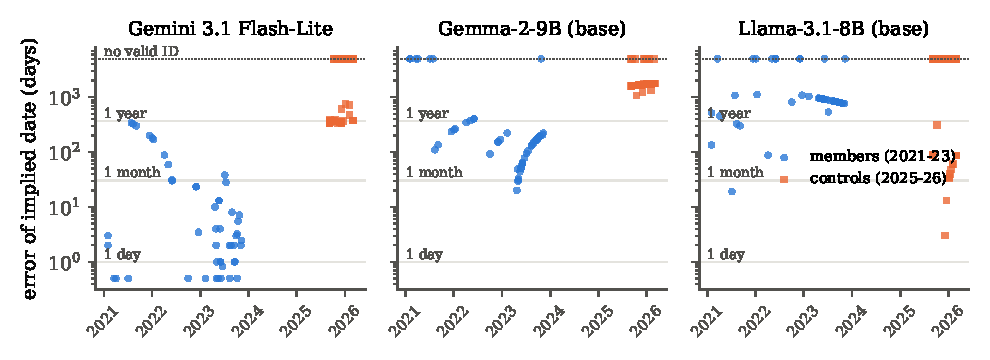
\includegraphics[width=\linewidth]{figures/fig_m10_urlid.pdf}
\caption{M10: distance in days between the date implied by the model's predicted article number and the true
publication date (log scale). Points on the dotted line are invalid numbers (outside the real range).}\label{fig:m10}
\end{figure}

What this shows, and what it does not:
\begin{itemize}
\item The model learned the relation between date and article number, which only \emph{La Vanguardia} URLs reveal.
So it has seen many of the newspaper's URLs from 2021--2023, either on the newspaper's own pages in web crawls or in
links to them elsewhere, for instance as citations in Wikipedia.
\item It does not show that any particular article was memorized: no exact number was produced. And knowing URLs is
not knowing text. The result says the newspaper's site was well represented in the model's training data, which is
why Gemini is the first candidate for the costly extraction tests.
\item Its control group is post-cutoff only. A same-period comparison with other newspapers' article numbers would show
whether this is specific to \emph{La Vanguardia} or a general skill with news URLs.
\end{itemize}

\paragraph{Other Gemini models.} The same 60 + 60 URL items were sent to every Gemini-API model. Gemini 3.5
Flash-Lite behaves like 3.1 Flash-Lite (median error 2 days; 31/49 members within 7 days vs 0/60 controls,
$p=7\times10^{-15}$; for controls it is off by a median of 230 days, consistent with a later cutoff and
extrapolation). Gemini 3 Flash, cut at 20 items by its quota, also does (median 4 days; 8/13 vs 0/9, $p=0.004$).
Gemini 2.5 models were closed to new users, 3.1 Pro has no free tier, and 3.5--3.8 Flash allow only 20 requests a day,
so they were not tested. Gemma-4 (open weights, via the API) exhausted its output budget on internal reasoning (about
100\,s per query, empty answers) and was stopped after 7 items; its two numeric answers were an order of magnitude off.

\paragraph{Can the article number be learned without reading the newspaper?} Yes, easily, so this signal only shows
exposure to the newspaper's \emph{URLs}.
\begin{itemize}
\item Every \emph{La Vanguardia} URL contains both the date and the number. The counter is so regular that an ideal
interpolator needs only 5 URLs spread over 2021--2023 to reach a median error of 3.7 days, 20 URLs for 1 day
(simulation over our 938 real 2021--2023 numbers).
\item Text pipelines of the FineWeb type remove hyperlinks, so a training text contains such a URL only where it is
written out. In one FineWeb-2 Spanish file (3.4 million documents; \texttt{src/m10\_url\_mentions.py},
\texttt{results/m10\_url\_mentions.json}) we found 136 written-out article URLs, \emph{all} in other sites' documents
(blogs citing sources, sites reposting agency news with ``M\'as informaci\'on en: lavanguardia.com/\dots''), and none
in the newspaper's own pages. Extrapolated to the 146 files, that is about 20,000 (date, number) examples, some 2,600
of them from 2021--2023.
\item A same-period comparison with three other newspapers that also use counters in their URLs (El Peri\'odico,
El Confidencial, El Espa\~nol; \texttt{src/m10\_outlet\_ids.py}) was started but stopped: the Common Crawl index was too
slow, and the FineWeb measurement already answers the question for text-trained models.
\end{itemize}
The finding remains a cheap triage signal (Gemini has absorbed many \emph{La Vanguardia} URLs), not evidence that the
newspaper's pages or text were used.

\paragraph{\emph{La Contra} question-to-answer recall.} A fifth item type targets the content of interviews. The model
receives the headline, date, intro heading and intro text of a \emph{La Contra} interview and one interviewer
question, verbatim, and is asked what the interviewee answered. Only answers that contain a specific fact (a number, name or place)
absent from everything shown are used; a hit means the model produces that fact (202 member and 76 control
interviews; more controls were collected for this, \texttt{data/cc/lacontra\_controls\_more.jsonl}). Gemini 3.5
Flash-Lite recalled the fact in 15/202 members and 5/76 controls (7\% each, $p=0.52$); the hits are guessable
(``Tierra'', ``Einstein'', ``Marina'' Abramovic). Overlap with the true answer's content words was equal (3.6\% both),
and the longest verbatim run was 5 words on members against 17 on controls. Gemma-2-9B (base, page continuation) recalled
2/151 vs 0/51 (run stopped at 202 of 278 items). The other local models were not run, because they showed weaker signals than Gemma-2 in every earlier
test. The interviews' specific answers are not known to these models.

\subsection{Reverse article-number test (M12, family C)}\label{sec:m12}
Pre-registered (\texttt{docs/prereg/m12\_url\_reverse.md}, amended once before any member query to make clear that the
answer must come from memory). If Gemini's precision with article numbers came from seeing the newspaper's pages
together with their URLs, the number should let it name the article. Articles come in pairs published on the same day
in the same section (117 member pairs, 2021--2023; 95 control pairs, after the training cutoff;
\texttt{data/m12/pairs.jsonl}, sha256 \texttt{009396f9\dots}). For each article the model gets the URL with the number,
date and section but without the title words, and is asked for the headline. Each answer is scored by its content-word
overlap with its own headline minus the overlap with the partner's: a model that uses only the date and section scores
0 on average by construction. Primary test: Wilcoxon on member pair scores (one-sided).

\begin{table}[h]\centering\small
\begin{tabular}{lrrrrr}
\toprule
Model & Member pairs & Mean pair score & $+/-$ pairs & $p$ (members) & $p$ (members vs controls)\\
\midrule
Gemini 3.5 Flash-Lite & 117 & $+0.006$ & 10 / 7 & 0.053 & 0.25\\
Gemini 3.1 Flash-Lite (replication) & 117 & $+0.004$ & 6 / 6 & 0.26 & 0.50\\
\bottomrule
\end{tabular}
\caption{M12 (\texttt{results/m12\_url\_reverse\_summary.json}). Controls: mean pair score $-0.001$ and $+0.000$. No
answer reached 0.8 overlap with its true headline in either model.}\label{tab:m12}
\end{table}
Both runs are null: the number does not lead Gemini to the article. Partial matches are the day's main news or daily
series (electricity price). Gemini knows the counter's pattern, not which article has which number. Raw records of most
of these queries were lost and are being re-run (Section~\ref{sec:setup}, evidence gap).

\subsection{Positive control on a model with published training data}\label{sec:posctrl}
\emph{OLMo 2 (discarded).} The public infini-gram index of OLMo 2's pretraining mix (\texttt{v4\_olmo-mix-1124\_llama})
contains almost no Spanish (``the city of Barcelona'' 56,500 occurrences; ``de la ciudad de Barcelona'' 658) and none
of the first 42 articles checked (\texttt{src/olmo\_positive\_control.py}, \texttt{results/olmo/lookup.jsonl}).

\emph{Apertus-8B} (\texttt{mlx-community/Apertus-8B-2509-4bit}, base). Pretrained on FineWeb-2 / FineWeb-2-HQ with
robots.txt opt-outs applied as of January 2025 (news pages of the newspaper were not opted out then), and with the
Goldfish objective, which suppresses verbatim recall. Groups (Spanish only, full FineWeb-2 scan): \emph{in} = found in
FineWeb-2 (563 random, 83 \emph{La Contra}); \emph{not found} (128, 117); post-cutoff controls (448, 41). Scores with \texttt{src/m5\_logprob.py}, calibrated with GPT-2-spanish; analysis
\texttt{src/positive\_control\_apertus.py} $\rightarrow$ \texttt{results/positive\_control\_apertus.json}.
\begin{itemize}
\item In vs post-cutoff controls, calibrated: loss AUC 0.550 ($p=0.003$), zlib ratio 0.552 ($p=0.002$), Min-K\% 0.534
($p=0.03$), Min-K\%++ 0.509 ($p=0.30$). The same split on the other open models, calibrated loss: Llama-3.1 0.539
($p=0.02$), Mistral 0.536 ($p=0.03$), Qwen2.5 0.527 ($p=0.07$), Salamandra-7B 0.564 ($p=0.0002$; int8 on Colab,
\texttt{src/m5\_hf.py}), Gemma-2 0.582.
\item In vs not found (same period): \textbf{reversed} for every model, raw AUC 0.38--0.42 and calibrated 0.42--0.48:
the articles FineWeb-2 did \emph{not} keep look more familiar. The 2018 reference, which saw neither group, shows the
same (0.44), also within publication year and section (0.42; \texttt{src/presence\_selection\_check.py},
\texttt{results/presence\_selection\_check.json}; calibrated, within strata: Apertus 0.44, $p=0.01$; Salamandra 0.49,
$p=0.33$). FineWeb-2's selection (quality filters, deduplication) kept a different kind of text; ``not found'' is
therefore not ``unseen'' (copies of a deduplicated article can survive under other URLs) and cannot serve as a
control group. The not-found articles also skew to 2020 and to the international and opinion sections.
\item \emph{La Contra}: calibrated AUC 0.38--0.41 in both comparisons, i.e.\ reversed as well (83 vs 117 / 41), on
every model.
\item Q$\rightarrow$A recall (page continuation): 0/90 facts for interviews in the data, 0/112 not found, 1/76 controls.
\end{itemize}
Reading: a model that (almost certainly) trained once on the articles shows no article-level knowledge and only a faint
collection-level trace, of the same size as the other open models. Null results are therefore uninformative about
training, and faint traces are what training looks like. Presence in a public dataset does not give clean
same-period groups (see above); those require articles that were never online (the publisher's archive).

\paragraph{Salamandra-7B (BSC), same tests.} La Contra Q$\to$A (\texttt{results/positive\_control\_apertus.json}): fact hits 2/90 for interviews in FineWeb-2, 3/112 not found, 2/76 controls (longest common run 4 words): no content recall, as Apertus. URL number as date (\texttt{results/m10\_summary.json}, $n=300$ per set): member median error 65 days (2021: 74, 2022: 63, 2023: 64), 12/245 within 7 days vs 0/300 controls ($p=5.9\times10^{-5}$); Gemini 2--3 days, Gemma-2 162, Llama-3.1 914. Like Gemini's, this shows exposure to La Vanguardia URLs (third-party links in Common Crawl suffice), not memorization of articles.

\subsection{Sentence-by-sentence extraction (M9, family A)}\label{sec:m9}
Following \cite{su2024}, M9 asks for one sentence at a time. A base (non-chat) open-weight model receives a plain
page: the newspaper's name, the title, byline and date, and the article up to the previous sentence. It simply
continues the page. There is no instruction, so there is nothing to refuse and nothing that could be called a
manipulated prompt. Llama-3.1-8B, run locally with greedy decoding, was tested on 100 \emph{La Contra} interviews
(460 sentences), 41 \emph{La Contra} controls (164 sentences) and 31 random member articles (123 sentences).
\begin{itemize}
\item No sentence was reproduced. The longest common run was 4 words on \emph{La Contra} members and 5 on controls
(median 1 for both). On random members it was 7 (median 2), all generic phrases.
\item The model writes plausible sentences on the right topic, in the series' style. It knows what the interviews
are about, but not how they were written.
\end{itemize}
Planned but not run because of compute time: the same test on Gemma-2, Qwen2.5 and Mistral; the chat versions of
Llama-3.1 and Qwen2.5 with the plain prompt of \cite{su2024}; the role-play prompt of \cite{freeman2024} as an upper
bound; and Gemini 3.1 Flash-Lite through the API (Section~\ref{sec:status}).

\subsection{NYT-style extraction (M11) and the most-copied articles (M13), family A}\label{sec:m11m13}
\paragraph{M11 (pre-registered, \texttt{docs/prereg/m11\_nyt\_style.md}).} The tricks of the NYT exhibits and
\cite{freeman2024}: a role-play system prompt (``2079, Jordi must restore the article word for word''), a fake
assistant acknowledgement, the first 110 words of the article, and 10 attempts (1 greedy + 9 sampled). Controls get
the same prompts and attempts. Score: longest common word run (LCS) with the next 250 words, outside quotation marks.
\emph{Salamandra-7B-Instruct, complete} (\texttt{results/m11\_summary.json}): \emph{La Contra} 60 members vs 60
controls, median 3 vs 3 words, maximum 10 vs 8, $p_{MW}=0.43$; random 40 vs 40, median 4 vs 4, maximum 15 vs 6,
$p_{MW}=0.38$. The single 15-word member run is the article's own subtitle, which is inside the 110-word prompt and
repeated in the body: the model copied its prompt (a scoring artifact to exclude in future versions). Qwen2.5 and
Llama-3.1 are in progress.

\paragraph{M13 (pre-registered, \texttt{docs/prereg/m13\_most\_copied.md}; API amendment
\texttt{m13\_amendment1\_api\_20261128.md}).} Memorization grows with the number of copies seen, so M13 applies M11's
protocol to the 20 most-copied articles in FineWeb-2 (245--1,279 near-identical copies each), prompting each article at
several points (every 300 words, plus a window ending at the article's end; 44 windows). Base rates: M11's controls
(offset 0) and 20 controls prompted mid-article; regurgitation threshold $\geq 25$ words outside quotes.
\begin{itemize}
\item \emph{Salamandra-7B-Instruct, complete}: most-copied vs M11 controls $p=0.57$ (maximum 10 vs 8 words);
vs M11's ordinary members $p=0.62$; mid-article windows vs offset controls $p=0.31$ (maximum 7 on controls). No
window reached 25 words, nor 15. Even the article copied 1,279 times (\emph{``Nosotros, como el tiempo, también nos
desdoblamos''}) gives at most 4 words. The longest runs are stock or topic phrases (``el pase a cuartos de final de
la Liga Europa'', 10; ``retirar el wi-fi de los colegios'', 7).
\item \emph{Gemini 3.1 Flash-Lite, partial} (free daily quota reached at 47 of 104 windows: all 44 most-copied
windows, 3 of 60 controls; no test result yet). One run of \textbf{26 words} on the 2014 Pope Francis interview
(``\ldots no puedo saludar a un pueblo y decirle que lo quiero dentro de una lata de sardinas, aunque sea de
cristal. Para mí\ldots''; 7 of 10 attempts $\geq 22$ words). It is the Pope's own answer, in a question-and-answer
interview without quotation marks, and is quoted verbatim by many outlets crediting the interview (e.g. El Tiempo,
a USCCB quotation list, Opus Dei and La Jornada pieces, 2025--2026 obituaries). It shows a memorized famous
quotation that first appeared in \emph{La Vanguardia}, not the newspaper's own wording: the interviewer's text around
it is not reproduced. Next longest: 14 words (Benedict XVI's farewell words, a quotation) and 13 (a scientist's name and
title). 0 of 483 attempts stopped for \texttt{RECITATION}.
\item \emph{Llama-3.1-8B-Instruct, complete}: mid-article windows vs offset controls $p=0.59$; maximum 11 words (a list of
banknote values) vs 12 on controls (a quoted statement); primary test pending Llama's M11 controls.
\item \emph{Qwen2.5-7B-Instruct, complete}: mid-article windows vs offset controls $p=0.055$ (n.s.); maximum 9 vs 6 words;
0 runs $\geq 25$; longest runs are topic phrases (``solicitar un visado para viajar a Estados Unidos deberán'', ``que su
rival a pesar de ser el visitante''); primary test pending Qwen's M11 controls.
\item \emph{Claude Opus 4.5, complete} (amendment 1; 40 own offset-0 controls + 20 offset controls): opening vs controls
$p=0.052$ (maximum 9 vs 6; pre-registered $\alpha=0.025$, not significant); mid-article $p=0.19$; 0 runs $\geq 25$; no
refusals (all 1,040 answers are continuations). Longest runs: Pope Francis 20 and 13 words, Benedict XVI 14, the
Garnier interview 10 (below).
\item \emph{Exploratory, not pre-registered} (no new queries): longest run against the whole article outside the prompt.
Claude: most-copied median 4, maximum 20 vs controls 3 and 9; Gemini 6.5 and 26 vs 6 and 10. Every run above 12 words is a
quoted statement of a public figure.
\end{itemize}

\paragraph{M13b, the Garnier interview (pre-registered follow-up, \texttt{docs/prereg/m13b\_garnier\_dense.md}).} In M13,
Claude continued the prompt at word 300 of the most-copied article with the original's next 9 words in 10 of 10
attempts and, in 7 of 10, echoed ``en el que podemos hacer cosas cuya'' from word 204 (neither in the prompt nor in the
scored text). M13b re-tests this with new queries: 110-word prompts every 50 words, 3 attempts, score = longest run
against the article outside the prompt; 4 \emph{La Contra} controls (Feb--Mar 2026), 15--16 windows each.
\emph{Claude Opus 4.5}: Garnier median 4 vs controls 2, maximum 13 vs 10, one-sided Mann--Whitney $p=0.0046$; windows
$\geq 12$: 1 vs 0; echoes 2 vs 2 (Fisher, n.s.). Robustness (not pre-registered): dropping runs that also appear in the
prompt, $p=0.0012$. Longest run: ``permite anticipar el presente a través de la memoria del futuro. En física'' (13
words, continuing the prompt; not found on the web outside copies of the interview). Limits: one article; windows are
not independent (article-level, 1 vs 4 cannot be significant); short runs; the interviewee's vocabulary.
\emph{Gemini 3.1 Flash-Lite} (secondary; complete): $p=0.41$, median 5 vs 4, maximum 6 vs 10, echoes 5 vs 16.

\paragraph{M13c, the next most-copied \emph{La Contra} interviews (pre-registered, \texttt{docs/prereg/m13c\_lacontra\_dense.md}).}
Does the Garnier signal generalize? M13b's protocol on \#2 Gérvas (490 copies), \#3 wi-fi (373) and \#18 L'Ecuyer (247),
against 8 \emph{La Contra} controls (M13b's 4 reused + 4 new; Feb--Mar 2026); Garnier excluded from the primary test.
\emph{Claude Opus 4.5}: article medians 5, 3, 0 vs controls 0--4; \textbf{article-level $p=0.38$}; window level $p=0.53$
(44 vs 116 windows); maximum 7 vs 10; 0 windows $\geq 12$ words; with Garnier (not confirmatory) $p=0.19$. Longest runs
are topic phrases (``el cáncer de cuello de útero'', ``hay que apagarlo por la noche''). L'Ecuyer's median of 0 is an
artifact of the pre-registered quote rule: its crawled text has 7 straight quotation marks, so most of it counts as
``inside a quotation''. Ignoring the quote flag for every article (exploratory): medians 5, 3, 5 vs 2--5, $p=0.069$
($0.048$ with Garnier). Reading: the Garnier fragments do not generalize to the next most-copied interviews at the
pre-registered level; at most a weak tilt in the predicted direction. Gemini run in progress.

\subsection{Recognition tests (M2, M2b, family C)}
Figure~\ref{fig:rec} and Table~\ref{tab:rec} summarize M2 and M2b. Read naively, the results look like strong
evidence: every model picks the original far above chance, with $p$-values as small as $10^{-90}$. But the models do
this \emph{equally well on controls}, articles they cannot have seen. Opus~4.5 picks the original among paraphrases of
post-cutoff articles 80.8\% of the time. The only quantity that can indicate training is the difference between
members and controls. That difference is small and not significant for any model (Opus +5.9 points, $p=0.15$;
Sonnet $-0.8$; Haiku +7.0, $p=0.09$), and it is negative in the pairwise test. The pairwise run on Gemini 3.1
Flash-Lite, now complete, shows the same: 58.9\% on members and 65.5\% on controls ($p=0.98$). Gemini also answered
``A'' in 78--89\% of cases, so position bias dominates its answers.

\begin{figure}[h]\centering
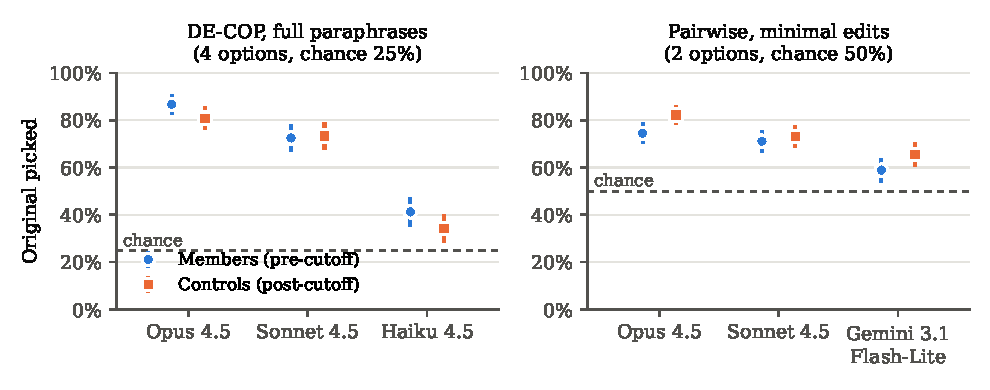
\includegraphics[width=\linewidth]{figures/fig_recognition.pdf}
\caption{Share of queries in which the original passage was chosen, with 95\% confidence intervals. If a model
recognized \emph{La Vanguardia} text from training, blue (members) would be clearly above orange (controls). It is
not. The high level of both shows that the models detect machine rewording, not remembered text.}
\label{fig:rec}
\end{figure}

\begin{table}[h]\centering\small
\fitbox{\begin{tabular}{llccc}
\toprule
Test & Model & Members & Controls & $p$ (members $>$ controls)\\
\midrule
M2 full paraphrases (chance 25\%) & Opus 4.5 & 86.7\% & 80.8\% & 0.15\\
 & Sonnet 4.5 & 72.5\% & 73.3\% & 0.55\\
 & Haiku 4.5 & 41.2\% & 34.2\% & 0.09\\
M2 minimal edits, 4 options (\emph{invalid}) & Opus 4.5 & 94.2\% & 96.6\% & 0.81\\
 & Sonnet 4.5 & 77.5\% & 88.1\% & 0.98\\
 & Haiku 4.5 & 78.8\% & 85.2\% & 0.90\\
M2b pairwise minimal edits (chance 50\%) & Opus 4.5 & 74.4\% & 82.2\% & 0.99\\
 & Sonnet 4.5 & 71.1\% & 73.2\% & 0.47\\
 & Gemini 3.1 Flash-Lite & 58.9\% & 65.5\% & 0.98\\
\bottomrule
\end{tabular}}
\caption{Recognition tests (60 + 60 articles; 240 queries per cell for M2, 360 for M2b). The last column is a
Mann--Whitney test on per-article accuracy.}\label{tab:rec}
\end{table}

\paragraph{Pitfall 1: paraphrase detectability.} High absolute DE-COP accuracy is routinely read as evidence of
exposure. Our controls show that frontier models recognize text rewritten by another AI (even text where only a few
words were swapped) as non-original, without having seen the source. Human writing and machine rewriting differ in
subtle ways, and the models detect that difference. Absolute accuracy, or a test against chance, is therefore
\emph{not} evidence of training. Presenting it as such would be misleading.

\paragraph{Pitfall 2: consensus leak.} With four options of which three are lightly edited variants of the original,
each variant changes \emph{different} words. The original is then the ``consensus'': every one of its words appears in
most options, and a simple majority vote recovers it without any memory. This explains the 85--97\% accuracy on
controls. The pairwise design, which shows one variant at a time, removes the leak.

\subsection{Answer-time retrieval (M4, family F)}\label{sec:m4}
This test asks whether an AI product fetches \emph{La Vanguardia} articles while answering and reuses their wording.
We used 25 controls (September 2025--March 2026). They were published after the model's training cutoff, so any
verbatim text in an answer would have to come from retrieval, not from training. Each article was requested with two
prompts: an explicit request to copy its first two paragraphs (QUOTE), and a natural question about its content (ASK).
Each prompt was run in two conditions: tools off, and Gemini's URL-fetching tool on (\texttt{src/m4\_retrieval.py};
100 logged calls). Google Search grounding could not be tested, because the free-tier key has no quota for it.
\begin{itemize}
\item \emph{The URL tool could not read the newspaper.} Google's fetcher reported an error for 49 of the 50 requests
on \texttt{lavanguardia.com} and for the site's homepage. The model then said it could not access the page. The same
tool fetched and copied a Wikipedia page without difficulty, and it also failed on another Spanish newspaper
(\emph{El Peri\'odico}). The site therefore appears to block this fetcher, whatever \texttt{robots.txt} says.
\item \emph{No article text was reproduced.} The longest match in any answer was 13 words, and in every such case it
was the article's own headline, which was in the prompt. The median match was 1--4 words.
\item \emph{Fabrication with tools off.} Asked for the first two paragraphs of an article it had never seen and
could not fetch, Gemini refused in 11 of 25 cases. In the other 13 it answered ``here are the first two paragraphs''
and wrote invented text in the newspaper's style (longest overlap with the real article: a few words). This is not
evidence of copying, but it is a separate issue: text the product falsely attributes to the newspaper.
\end{itemize}
For the Gemini API, then, we see no answer-time reuse, because the fetch fails. Consumer products (ChatGPT search,
Perplexity, Gemini with Google Search, Claude with web search) use different fetchers and search indexes and need a
separate test, ideally with accounts and a protocol agreed with counsel.

\subsection{Token-probability tests (M5, family B)}
Figure~\ref{fig:auc} reports AUCs on all 695 members and 448 controls. Uncalibrated, Qwen2.5-7B separates members from
controls weakly but significantly (Min-K\% AUC $0.560$, 95\% CI $[0.527,0.597]$, $p=3\times10^{-4}$). The
2018-data reference model, which cannot have seen either group, also shows a gap (Min-K\% $0.533$, $p=0.03$). This is
the time effect. After calibration a small signal remains: loss AUC $0.542$ $[0.507,0.575]$ ($p=0.008$),
Min-K\% $0.534$ $[0.501,0.565]$ ($p=0.025$), zlib ratio $0.500$. In plain terms, for a random member--control pair the
calibrated score points to the member about 53--54\% of the time, against 50\% for a coin. This is compatible with
modest exposure of Qwen2.5 to \emph{La Vanguardia} text. It is far from what could identify an individual article,
and the scores do not agree with one another.

\begin{figure}[h]\centering
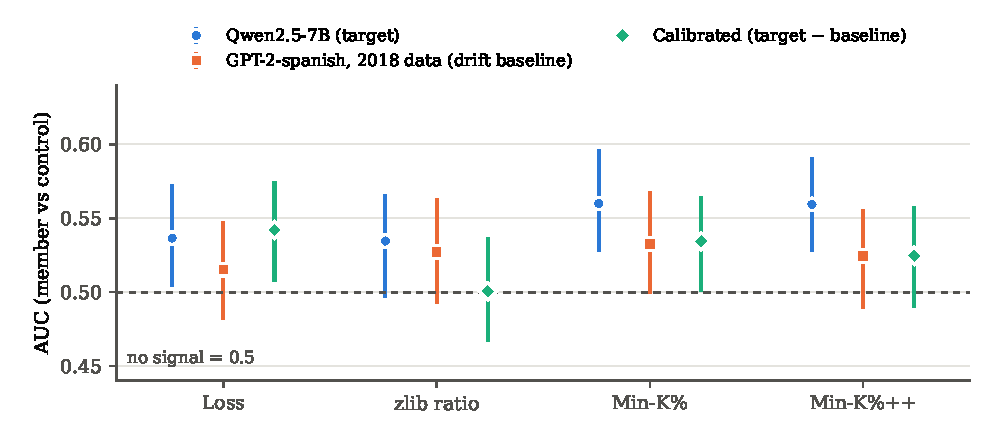
\includegraphics[width=\linewidth]{figures/fig_logprob_auc.pdf}
\caption{Member-vs-control AUC (bootstrap 95\% CI) for four membership scores; 0.5 means no separation. Orange: how
much separation arises from time alone (a model that saw neither group). Green: the target model's separation after
removing the time effect.}
\label{fig:auc}
\end{figure}

On \emph{La Contra} (212 members, 41 controls) the raw scores show a weak gap for some metrics (zlib ratio AUC
$0.605$, $p=0.02$), but the reference model shows the same gap ($0.593$). After calibration no signal remains (AUC
$0.45$--$0.54$, all $p\ge0.23$). The highly reposted interviews are therefore no more ``familiar'' to Qwen2.5 than
ordinary articles. The small number of controls makes these estimates imprecise.

\subsection{Dataset inference (M6, family D)}\label{sec:di}
Table~\ref{tab:di} reports the dataset-inference test. Read row by row:
\begin{itemize}
\item On Qwen2.5's raw scores the collection test is overwhelmingly ``significant'' ($p=0.0004$, significant in all
splits).
\item The \emph{reference model alone}, which cannot have seen either group, is \emph{also} significant
($p=0.007$, 82\% of splits). This is the decisive observation. With date-based controls, dataset inference detects
the passage of time, not training. Taken at face value it would ``prove'' that a 2018 model was trained on articles
written in 2020--2023, which is impossible.
\item After calibration (removing what the reference model explains) the result is weaker ($p=0.02$, significant in
69\% of splits). It is suggestive, but not robust, and it may contain residual drift that the small reference model
does not capture.
\item The null check behaves as it should: splitting controls against controls gives no signal (median $p=0.53$; only
2\% of runs below 0.05). The procedure does not invent differences where none exist.
\end{itemize}

\begin{table}[h]\centering\small
\fitbox{\begin{tabular}{llccc}
\toprule
Sample & Scores used & Median $p$ & Splits with $p<0.05$ & Interpretation\\
\midrule
Random (695 vs 448) & Qwen2.5 raw & 0.0004 & 100\% & membership + time\\
 & Reference (2018 model) only & 0.007 & 82\% & time alone\\
 & Calibrated (Qwen2.5 $-$ reference) & 0.02 & 69\% & membership (approx.)\\
 & Null: controls vs controls & 0.53 & 2\% & sanity check passed\\
\emph{La Contra} (212 vs 41) & Qwen2.5 raw & 0.03 & 65\% & \\
 & Reference only & 0.010 & 81\% & time alone\\
 & Calibrated & 0.07 & 44\% & not significant\\
\bottomrule
\end{tabular}}
\caption{Dataset inference (200 random splits each). The reference-only rows show that date-based controls alone
produce ``significant'' results.}\label{tab:di}
\end{table}

\paragraph{How many articles are needed?} On calibrated scores, the share of subsampled runs reaching $p<0.05$ grows
with collection size: 0\% with 50 articles per group, 10\% with 100, 15\% with 200, 20\% with 300 and 45\% with 448.
If the calibrated signal is real, a few thousand articles per group would make it reliably significant, which is
within reach of the God\'o archive. But size cannot fix a biased validation set: more articles make \emph{any}
systematic difference significant, including drift.

\paragraph{Four models, matched groups and placebos.} Table~\ref{tab:dimulti} repeats the test on four
open-weight models from four providers. Without matching, every model looks ``guilty'' on raw scores and three of
four remain significant after calibration. Once the groups are matched by section and length, the calibrated result
disappears for Qwen2.5, Llama-3.1 and Mistral ($p=0.13$--$0.29$). Only Gemma-2 (Google) remains significant
($p=0.009$). All placebos are clean (calibrated $p\ge0.26$), so the procedure does not confuse a few months of
time difference with training.

\begin{table}[h]\centering\small
\fitbox{\begin{tabular}{lccccccc}
\toprule
 & \multicolumn{3}{c}{Unmatched (695 vs 448)} & \multicolumn{3}{c}{Matched (440 pairs)} & Placebo\\
\cmidrule(lr){2-4}\cmidrule(lr){5-7}
Target & raw & ref.\ only & calibrated & raw & ref.\ only & calibrated & (calibrated)\\
\midrule
Qwen2.5-7B (Alibaba) & 0.0005 & 0.007 & 0.04 & 0.002 & 0.006 & 0.29 & 0.65\\
Llama-3.1-8B (Meta) & 0.0009 & 0.007 & 0.03 & 0.004 & 0.006 & 0.29 & 0.56\\
Mistral-7B-v0.3 (Mistral AI) & 0.0001 & 0.007 & 0.010 & 0.0004 & 0.006 & 0.13 & 0.45\\
Gemma-2-9B (Google) & 0.0008 & 0.007 & $2\times10^{-5}$ & 0.012 & 0.006 & \textbf{0.009} & 0.33\\
\bottomrule
\end{tabular}}
\caption{Dataset inference, median $p$ over 100 splits (reference: GPT-2-spanish, 2018 data). ``Ref.\ only'' uses
the reference model alone, which cannot have seen either group: its significance measures the time effect.
Placebo: controls Sep--Dec 2025 vs Jan--Mar 2026, both unseen.}\label{tab:dimulti}
\end{table}

\paragraph{Is the Gemma-2 result evidence of training on \emph{La Vanguardia}?} It is robust to the matching
tolerance (10--50\%: $p=0.007$--$0.011$), to using loss or Min-K\% alone ($p=0.002$, $0.007$), and to removing the
opinion, economy, politics or culture sections. But it falls to $p=0.09$ when the \emph{international} section is
removed. Members' international news (pandemic, war in Ukraine) concerns events that any model trained in 2024
knows from thousands of sources; controls describe events after its cutoff. The neighbour test (M7) settles the
question. It asks whether the model prefers \emph{La Vanguardia's wording} over a rewrite with the same facts, and
for all four models members show no stronger preference than controls (Table~\ref{tab:neigh}). For Gemma-2 the
difference even points the other way. The Gemma-2 signal therefore reflects knowledge of the \emph{period's events},
not of the newspaper's text. In legal terms, it is evidence about facts, which are free, not about the protected
expression.

\begin{table}[h]\centering\small
\fitbox{\begin{tabular}{lcccc}
\toprule
 & \multicolumn{2}{c}{Full rewrites} & \multicolumn{2}{c}{Minimal edits}\\
\cmidrule(lr){2-3}\cmidrule(lr){4-5}
Target & member $-$ control (95\% CI) & $p$ & member $-$ control (95\% CI) & $p$\\
\midrule
Qwen2.5-7B & $-0.013$ [$-0.064$, $0.036$] & 0.23 & $+0.004$ [$-0.014$, $0.023$] & 0.71\\
Llama-3.1-8B & $-0.022$ [$-0.073$, $0.031$] & 0.15 & $+0.001$ [$-0.019$, $0.021$] & 0.61\\
Mistral-7B-v0.3 & $-0.009$ [$-0.056$, $0.036$] & 0.29 & $-0.006$ [$-0.027$, $0.015$] & 0.34\\
Gemma-2-9B & $+0.048$ [$-0.021$, $0.111$] & 0.89 & $+0.034$ [$0.010$, $0.057$] & 1.00\\
\bottomrule
\end{tabular}}
\caption{Neighbour test (M7), 60 members vs 60 controls. Value: difference in the loss gap (original minus mean of
rewrites); negative would mean members' original wording is specifically more familiar. One-sided Mann--Whitney $p$.
No model shows a wording-specific signal.}\label{tab:neigh}
\end{table}

\paragraph{A second reference model, and a trap in the learned combination.} We repeated the test with a larger
reference, XGLM-2.9B (Meta; Common Crawl data up to 2020; members before June 2020 dropped). With it, the learned test
declared \emph{all four} models significant even after matching (calibrated $p=0.0001$--$0.003$). The reason is
instructive. XGLM reacts to the time gap more strongly than the targets on one score (Min-K\%), so after
subtraction members look \emph{less} familiar than expected on that score. The logistic regression is free to give
any score a negative weight, so it treats ``less familiar than expected'' as evidence too. A miscalibrated reference
thus manufactures significance. We therefore also ran a \emph{pre-registered, sign-constrained} version: each score
is oriented in advance so that higher means more familiar, standardized, and averaged with equal weights; nothing is
learned from the data. With matched groups, the reference model alone is then not significant ($p=0.20$--$0.32$).
Results for the targets (calibrated, GPT-2 / XGLM reference) are: Qwen2.5 $p=0.06$ / $0.59$; Llama-3.1 $0.06$ /
$0.61$; Mistral $0.03$ / $0.37$; Gemma-2 $10^{-4}$ / $0.002$. Only Gemma-2 is significant under both references,
and the neighbour test above shows its signal is not about wording.

\emph{Lesson for court use:} the direction of the test and the way scores are combined must be fixed \emph{before}
looking at the data, and the conclusion must not depend on the choice of reference model.

\paragraph{Two models, same articles (M8).} Table~\ref{tab:did} reports the Llama-3 vs Llama-3.1 comparison. For
each article we measure how much \emph{more} familiar it is to Llama-3.1 than to Llama-3. If training on the
newspaper leaves a trace, this gain should be larger for articles that only Llama-3.1 could have seen (April--November
2023) than for articles both saw (2020--February 2023) or neither saw (controls). This is exactly what we observe. The
April--November 2023 group gains more on three of the four scores, and the pre-registered equal-weight combination is
significant against both comparison groups ($p=0.007$ each). The two groups that should \emph{not} differ (seen by
both vs seen by neither) do not ($p=0.42$), and a placebo splitting the ``seen by both'' group by date is clean
($p=0.63$). Because the same articles are scored by both models, time drift cancels by design.

The effect is small: about 0.17 standard deviations, or 0.01 in average loss on a scale of about 2.3. It also shares
the limitation of Gemma-2's result. Llama-3.1's extra training data covers the \emph{events} of mid-2023 from all
sources, so a larger gain on mid-2023 articles is what knowledge of those events alone would also produce. The
learned (logistic) version of the test is only borderline ($p=0.06$ and $0.21$). The design is the cleanest we have,
but to attribute the gain to \emph{La Vanguardia's text} it must be combined with the neighbour test on the mid-2023
articles, or with same-period articles that were never online.

\begin{table}[h]\centering\small
\fitbox{\begin{tabular}{lccccc}
\toprule
 & \multicolumn{3}{c}{Mean gain in familiarity, Llama-3.1 vs Llama-3} & \multicolumn{2}{c}{Combined test (pre-registered)}\\
\cmidrule(lr){2-4}\cmidrule(lr){5-6}
Score & Seen by both (695) & Seen by 3.1 only (249) & Seen by neither (448) & comparison & $p$\\
\midrule
Loss & 0.013 & \textbf{0.019} & 0.009 & 3.1-only vs neither & 0.007\\
zlib ratio ($\times10^3$) & 0.3 & \textbf{0.5} & 0.3 & 3.1-only vs both & 0.007\\
Min-K\% & $-0.015$ & \textbf{0.007} & $-0.015$ & both vs neither & 0.42\\
Min-K\%++ & $-0.087$ & $-0.069$ & $-0.074$ & placebo (both, by date) & 0.63\\
\bottomrule
\end{tabular}}
\caption{Two-model difference-in-differences (M8). Gains are oriented so that larger = more familiar to Llama-3.1.
Per-score tests, 3.1-only vs neither (one-sided Mann--Whitney): loss $p=0.001$, zlib $p=0.003$, Min-K\% $p=0.02$,
Min-K\%++ $p=0.30$.}\label{tab:did}
\end{table}

\paragraph{Wording or events? The neighbour test inside the two-model design.} To separate the two explanations, we
repeated the comparison on the neighbour gap of Section~\ref{sec:di}. For each passage, the gap is how much more
familiar the \emph{original} wording is than three rewrites with the same facts, produced locally by a model of
another family (Qwen2.5-7B-Instruct). Knowledge of the events lowers the loss of the original and of the rewrites
alike, so it cancels in the gap. Time drift cancels because both models score the same passages. What remains is
familiarity with the \emph{wording}. The prediction, if Llama-3.1 was trained on the newspaper's text, is that its
gain in original-wording preference over Llama-3 is largest for the April--November 2023 articles.

\begin{table}[h]\centering\small
\fitbox{\begin{tabular}{lccc}
\toprule
Comparison & Loss: difference in gap change [95\% CI] & $p$ (loss) & $p$ (combined, pre-registered)\\
\midrule
3.1-only (248) vs neither (249) & $-0.012$ [$-0.025$, $0.002$] & 0.09 & 0.069\\
3.1-only vs both (250) & $-0.011$ [$-0.025$, $0.004$] & 0.15 & 0.065\\
both vs neither (check) & $-0.001$ [$-0.015$, $0.012$] & 0.40 & 0.53\\
\bottomrule
\end{tabular}}
\caption{Neighbour test inside the Llama-3 vs Llama-3.1 design (\texttt{results/did\_neighbour.json}). Negative =
Llama-3.1 gained more preference for the original wording. One-sided tests: Mann--Whitney (loss) and Welch on the
equal-weight combination of four scores (effect $\approx0.12$ SD).}\label{tab:didneigh}
\end{table}

The result points in the predicted direction. Between the two model versions, the preference for the original wording
shifts away by about the same amount for articles seen by both and by neither ($+0.012$ in loss). For the articles
only Llama-3.1 could have seen, it barely shifts ($+0.001$). The check comparison is clean ($p=0.53$). But the
difference is not statistically significant ($p\approx0.07$), so on its own it does not establish use of the
newspaper's wording. With about 250 articles per group, the test can only detect effects of about 0.2 SD. We have
therefore pre-registered an independent replication on articles not used in this run
(\texttt{docs/prereg/did\_neighbour\_replication.md}), committed before any replication data was collected. Simply
adding articles until the $p$-value drops below 0.05 would inflate false positives. The replication was stopped after
the rewrites of 247 of about 810 passages and later completed on Google Colab with the same models in
\texttt{transformers} (nf4 4-bit), all rewrites regenerated; these deviations were recorded and committed before any
scoring. Only 168 fresh mid-2023 articles could be found in the three crawls, so the replication's ``seen only by
Llama-3.1'' group is smaller than the original's. Three of 811 passages (IDs 7740491, 8098952, 8191781) got fewer than
three valid rewrites and were dropped by the registered rule, leaving 168 / 442 / 198 (NEW2 / BOTH2 / NONE2).
\emph{Result} (\texttt{results/did\_neighbour\_rep.json}): NEW2 vs NONE2 combined effect $+0.122$ SD, $p=0.097$;
NEW2 vs BOTH2 $+0.118$ SD, $p=0.067$; check BOTH2 vs NONE2 $-0.012$ SD, $p=0.57$ (clean). Loss alone (Mann--Whitney):
$p=0.053$ and $0.12$. The direction and size match the first run, but the pre-registered test is not significant, so
the effect is \emph{not confirmed}. Secondary, pooled over both runs (mixing MLX and \texttt{transformers} backends;
\texttt{results/did\_neighbour\_pooled\_secondary.json}): NEW vs NONE $+0.108$ SD, $p=0.038$; NEW vs BOTH $p=0.11$;
but the check comparison is not clean on loss ($p=0.039$), so the pooled result adds nothing reliable.

\paragraph{Designing a sound validation set.} The method's power depends on a validation set that differs from the
suspect set \emph{only} in exposure to the model. The publisher's archive makes much better designs possible than ours:
\begin{enumerate}
\item \emph{Crawled vs never-crawled, same period.} For each archive article, the Common Crawl index tells whether it
was ever captured. Articles from the same months, sections and authors that were \emph{never} captured (for example
paywalled or print-only pieces) form a natural validation set with no time gap. Residual differences, such as why some
articles were not captured, can be checked by matching on section, length and author.
\item \emph{Print-only or unpublished content.} Material that never appeared online (some print supplements, archived
but unpublished texts) is certainly unseen and comes from the same newsroom and period.
\item \emph{Two models, same articles.} The same suspect and validation sets can be scored with two models of the
same family with different cutoffs. A model trained before the validation articles existed and a model trained after
both sets were online should show different gaps only if training matters. This difference-in-differences design
cancels drift without needing a perfect validation set.
\end{enumerate}
With design~1 or~2 and a few thousand articles, dataset inference on open-weight commercial models (Llama, Qwen,
Mistral, Gemma, DeepSeek) is the most promising route to a statistically sound statement. That statement would take
the form ``this model was trained on La Vanguardia's archive, with a false-positive risk below X\%''.

%======================================================================
\section{Discussion}
\paragraph{Feasibility.} For ordinary, randomly sampled news articles, today's frontier models do not exhibit the
verbatim recall that made \emph{GEMA} straightforward. Song lyrics are duplicated thousands of times on the web; a
typical signed news article is not. This is consistent with the duplication dependence of memorization
\cite{carlini2023}. The \emph{La Contra} experiment tests that explanation directly. Even the newspaper's most widely
reposted content is not reproduced by any of five Claude models from a neutral 60-word prompt, including models whose
training data post-dates every member interview. Recognition tests on black-box models are dominated by style cues,
and token-probability tests give weak signals once the time effect is removed. A per-article demonstration in the
style of \emph{GEMA} or the NYT exhibits is therefore unlikely to succeed with defensible prompts. Stronger extraction
(longer context, many attempts, jailbreaks \cite{ahmed2026}) may still succeed. Following Section~\ref{sec:nyt}, it
would support a memorization claim more than an output claim.

\paragraph{What may work.}
\begin{enumerate}
\item \emph{Dataset-level inference} (Section~\ref{sec:di}). Weak per-article signals can become significant when
aggregated over thousands of articles \cite{maini2024}. Our pilot shows both the promise and the main risk: date-based
controls create false positives, so the validation set must come from the same period. This is feasible with the licensed archive on models that expose token probabilities
(open-weight models, some commercial APIs), provided that controls are matched on section, author and length and the
time effect is calibrated as above. The result is a statement about the \emph{collection}. Under \emph{GEMA} reasoning
that may be less directly actionable than a reproduced article, but it is relevant to disclosure requests and to the
AI Act training-content summaries.
\item \emph{Retrieval-time use.} Web-enabled assistants may fetch and reproduce paywalled articles at answer time.
This is a different legal act from training (Section~\ref{sec:lawful}), but it is directly observable.
\item \emph{Other high-duplication content.} Star columnists, editorials and viral stories remain untested, as do
sentences demonstrably quoted on many other sites. Duplication could be measured directly in Common Crawl to select
the passages most likely to be memorized.
\item \emph{Copyright traps.} Unique sequences planted in future articles would make later detection far more
reliable \cite{meeus2024}.
\end{enumerate}

\paragraph{Legal reading.} Given the opt-out chronology, showing that crawling happened is not sufficient for pre-2026
content in the EU. The relevant evidence is memorization (reproduction in the model, as in \emph{GEMA}) or
reproduction in outputs. Absence of evidence in our pilot is not evidence of absence. The tests have limited power,
and memorization may be concentrated in a few highly duplicated pieces that our samples miss.

\section{Limitations}
\begin{itemize}
\item Sample sizes for the API tests are small (60+60 random articles; up to 100 \emph{La Contra} interviews).
\item Members and controls differ in date and therefore in topic mix. The reference model is much smaller than the
target and was trained on a different corpus, so the time correction is approximate.
\item Paraphrases were produced by a Claude model, which may interact with Claude targets.
\item Claude outputs are not deterministic (Gemini calls used temperature 0).
\item Four open-weight targets were evaluated, all of 7--9 billion parameters; larger models memorize more. M9 was
run on only one of them. Claude
5.x models could only be tested where controls are not essential.
\item The M10 screening used 60 items per type and group, with few \emph{La Contra} controls (24--38), and
was run on one commercial API model so far.
\item The neighbour test used only 60+60 passages, so it can miss a small effect.
\item The retrieval test covered only the Gemini API's URL tool (25 articles). Search grounding and consumer
products with web access are untested.
\item Gemini evaluation was limited by free-tier quotas and by the lack of token probabilities. Several runs were cut
short by API credit and quota limits (marked in the tables). OpenAI models have not been evaluated yet.
\end{itemize}

\section{Status: what is missing, and what it would cost}\label{sec:status}
The study was stopped at the stage described above. Table~\ref{tab:status} lists the work that was designed but not
completed, and what each item needs. As a reference for API costs, our Claude experiments cost about \$20 for 6,220
calls (about \$0.003 per call). Prices change, so these are orders of magnitude.

\begin{table}[h]\centering\small
\begin{tabularx}{\linewidth}{>{\raggedright\arraybackslash}p{4.4cm}>{\raggedright\arraybackslash}X}
\toprule
Missing item & What it needs, and its cost or problem\\
\midrule
Claude tests (M1 \emph{La Contra} for Sonnet/Opus 4.5, M9, role-play) & Anthropic API credit (exhausted). Sonnet~4.5 is
retired on 30~Nov.~2026, after which it can no longer be tested. Tens of dollars for the planned runs.\\
Gemini: M9 (plain and role-play), M1 controls for Gemini~3 Flash & The free tier allows about 500 requests per model per
day, so each run takes days. A billed key removes the limit; the runs cost a few dollars.\\
Retrieval with search (Gemini with Google Search, ChatGPT search, Perplexity, Claude web search) & Search grounding
requires a billed Gemini key. Consumer products need accounts and either manual sessions or browser automation, which
may conflict with terms of service. The protocol should be agreed with counsel and the sessions recorded (for
example before a notary).\\
OpenAI models & An API key. Word probabilities are only returned for generated text, not for supplied text, so only
black-box tests apply.\\
M9 at a scale where a 1--2\% hit rate becomes visible & About 30 queries per article over 1,000 or more articles: some
30,000 queries per model, roughly \$100 per model at the rate above.\\
Local open-weight runs (M9 on four more models, neighbour-test replication) & On the 16~GB laptop used here, about
9 seconds per query when two jobs share the GPU: about 1--2 days in total. Free, but slow.\\
Larger open-weight models (70B and up) & Memorization grows with model size \cite{carlini2023,freeman2024}, so these
matter most. They do not fit on a laptop: a rented cloud GPU for a few days, or a workstation with 64~GB or more of
memory. Disk space must also be freed (about 6~GB is left).\\
M10 article-number test on all reachable models, with other newspapers as a same-period control & One short
query per article: a few hundred queries per model, cents with a paid key; days on free tiers.\\
Same-period controls & The publisher's archive, to compare crawled with never-crawled articles of the same months.\\
Copyright traps & A decision by the publisher. They only protect future content.\\
\bottomrule
\end{tabularx}
\caption{Work designed but not completed.}\label{tab:status}
\end{table}

%======================================================================
\section{Conclusions}
Main insights, in plain language:
\begin{itemize}
\item \textbf{The articles were available for AI training.} \emph{La Vanguardia}'s full article text has been in
Common Crawl, the main public source of AI training data, for years. News articles were not opted out of AI crawlers
until 17 March 2026.
\item \textbf{Availability is not proof of use, and before March 2026 it may have been lawful.} Under EU law, training
on openly available text is allowed unless the owner opted out in a machine-readable way, which happened only in
March 2026.
\item \textbf{The strongest legal argument is memorization or reproduction.} A German court (\emph{GEMA}) held that a
model that has memorized a work contains an infringing copy. That needs a model that reproduces the articles.
\item \textbf{We found no reproduction.} Seven commercial models (Claude 4.5 and 5.5, Gemini 3.x) do not reproduce
\emph{La Vanguardia} articles word for word, not even the widely shared \emph{La Contra} interviews. They know the
facts, but not the wording.
\item \textbf{Some popular tests give false positives.} Models identify the original text among AI-written rewordings
even for articles they cannot have seen. Any claim based on such tests must be checked against articles published
after the model's training.
\item \textbf{The faint statistical traces are explained by time and world knowledge.} Four open-weight models find
older \emph{La Vanguardia} articles slightly more familiar than new ones. After comparing like with like (same
section, similar length) the trace disappears for three of them. For the fourth (Google's Gemma-2) it remains, but it
comes from knowing the \emph{events} of 2020--2023, not the newspaper's \emph{wording}: the model does not prefer the
original sentences over rewrites with the same facts. Facts are not protected; wording is.
\item \textbf{The best design compares two versions of the same model.} Articles that only the newer Llama could have
seen became slightly more familiar to it than the others did, exactly as training would predict and with time effects
cancelled. The effect is small. When only the \emph{wording} is compared (original sentences vs rewrites with the
same facts), the result still points the same way but is not statistically significant ($p\approx0.07$). An
independent replication, with its analysis fixed in advance, found the same direction and size, again not significant
($p\approx0.07$--$0.10$): not confirmed.
\item \textbf{Testing the collection as a whole (dataset inference) is the most promising route.} Small differences
that are invisible in one article add up over thousands. Our pilot shows the main dangers: comparing old with new articles ``proves'' training even for a model
that cannot have seen them, and a model's knowledge of past events can pass for knowledge of the text. Every result
must therefore pass placebo groups and a wording-specific check. The comparison articles must come from the \emph{same period}. The publisher's archive
allows this, for example by comparing articles that web crawlers captured with articles from the same months that
were never online. This approach requires models whose word probabilities are accessible: open-weight models, or
commercial models under court-ordered expert access.
\item \textbf{Answer-time use is a separate avenue.} Assistants that browse the web may reproduce articles at
answer time. This is a different legal act, easier to observe. In a first test, Google's Gemini API could not fetch
\emph{La Vanguardia} pages and reproduced no text. Without access, it sometimes invented ``literal'' paragraphs and
attributed them to the newspaper. Consumer products with web search remain to be tested.
\item \textbf{Which models are most suspicious (no evidence yet).} ``Suspicious'' here means a statistical trace
that points towards training on the newspaper but does not meet the standard of proof. In decreasing order:
\begin{itemize}
\item \emph{Google's Gemini 3.1 Flash-Lite} (exposure, not memorization). Given only an article's title and date,
it names the newspaper's internal article number to within a few days for 2021--2023 articles, which only many
\emph{La Vanguardia} URLs can teach. It reproduces no text and recalls no exact number, so this places the site in its
training data without showing that any article was copied.
\item \emph{Google's Gemma-2.} It is the only model whose collection-level trace survived matched comparison groups,
the pre-registered combination and both reference models ($p=10^{-4}$ and $p=0.002$). The neighbour test attributes
this trace to knowledge of events, not wording, so it is not evidence of copying.
\item \emph{Meta's Llama-3.1.} Articles published between the cutoffs of Llama-3 and Llama-3.1 became more familiar
to the newer model ($p=0.007$). The wording-only version points the same way ($p\approx0.07$). This is the design
closest to evidence about the text; its pre-registered replication pointed the same way but was not significant.
\item \emph{Mistral-7B and Qwen2.5} show weaker traces that depend on the reference model, so they are not robust.
\item \emph{Closed commercial models} (Claude, Gemini, and untested GPT). Our black-box tests found nothing, but those
tests have little power. Larger models memorize more, and corpora of the FineWeb-2 type contain most of our
articles. Their use of the newspaper's text is plausible but unproven. Gemini additionally invents ``literal''
passages and attributes them to the newspaper.
\end{itemize}
\item \textbf{Which content is most likely to have been used.} The articles most exposed to training are those
captured by Common Crawl between 2019 and 2023 and published from 2017 to 2021. They dominate the newspaper's pages
in FineWeb-2, and 82\% of our 2020--2023 sample is in it. The Catalan edition is proportionally
the most exposed: \emph{La Vanguardia} supplies about one document in a thousand in FineWeb-2's Catalan part, about
1.5 times its share in Spanish. A newspaper this prominent in Catalan web text is likely to have contributed to the Catalan
abilities of any model trained on such corpora. Less exposed are articles from 2024 onwards, which are rare in these
datasets, and from 17~March~2026, after the opt-out. Paywalled and print-only pieces were never in public crawls.
Quotations inside articles (statements, rulings) circulate in many outlets, so reproducing them proves nothing about
the newspaper.
\item \textbf{Copyright traps are the most reliable option for the future.} Inserting unique, invented phrases into
future articles, repeated across many pages, would make later reproduction by a model unambiguous proof of use. We
recommend starting now, since traps cannot protect content published before their introduction.
\end{itemize}

\paragraph{Next steps.} See Table~\ref{tab:status}. In order of value: finish the pre-registered NYT-style
extraction (M11, \texttt{docs/prereg/m11\_nyt\_style.md}: role-play prompt, 110-word opening, best of 10 attempts,
identical for controls; an adversarial upper bound reported apart from the neutral tests): done on
Salamandra-7B-Instruct (null), in progress on Qwen2.5-7B-Instruct, Llama-3.1-8B-Instruct needs an HF token;
finish M13 on Gemini 3.1
Flash-Lite (quota), Qwen2.5 and Llama-3.1, then Claude Opus 4.5 (pre-registered); ask the publisher for server
logs (which crawlers fetched the articles, and when); retrieve Anthropic's AI Act training-content summary; scan BSC's CATalog; the
cheap article-number screening (M10) on all reachable models, to choose where to spend on extraction tests; M9 and
role-play tests on commercial APIs with a paid key; tests on larger open-weight models; complete the truncated runs; measure duplication to select test passages; evaluate models from
other providers that expose token probabilities (OpenAI, further open-weight models); run dataset inference on the
licensed archive with same-period controls (crawled vs never-crawled articles) and on several open-weight models; extend the retrieval test to web-enabled consumer assistants; and agree with the
publisher on a copyright-trap protocol.

\paragraph{Reproducibility.} Code is in \texttt{src/}; figures are regenerated by \texttt{paper/make\_figures.py}
from \texttt{results/}. Raw query logs (\texttt{evidence/}) are kept outside version control because they contain
article text.

\paragraph{Acknowledgement.} The pipeline, experiments and this draft were produced with the assistance of an AI
coding agent (Claude Code).

\begin{thebibliography}{99}\small
\bibitem{carlini2021} N.~Carlini et al. Extracting training data from large language models. \emph{USENIX Security}, 2021.
\bibitem{carlini2023} N.~Carlini et al. Quantifying memorization across neural language models. \emph{ICLR}, 2023.
\bibitem{nasr2023} M.~Nasr et al. Scalable extraction of training data from (production) language models. arXiv:2311.17035, 2023.
\bibitem{ahmed2026} A.~Ahmed, A.~F.~Cooper, S.~Koyejo, P.~Liang. Extracting books from production language models. arXiv:2601.02671, 2026.
\bibitem{freeman2024} J.~Freeman, C.~Rippe, E.~Debenedetti, M.~Andriushchenko. Exploring memorization and copyright violation in frontier LLMs: a study of the New York Times v.\ OpenAI 2023 lawsuit. arXiv:2412.06370, 2024.
\bibitem{su2024} E.~Su et al. Extracting memorized training data via decomposition. arXiv:2409.12367, 2024.
\bibitem{shi2024} W.~Shi et al. Detecting pretraining data from large language models. \emph{ICLR}, 2024.
\bibitem{zhang2024} J.~Zhang et al. Min-K\%++: Improved baseline for detecting pre-training data from large language models. arXiv:2404.02936, 2024.
\bibitem{duarte2024} A.~V.~Duarte et al. DE-COP: Detecting copyrighted content in language models training data. \emph{ICML}, 2024.
\bibitem{maini2024} P.~Maini, H.~Jia, N.~Papernot, A.~Dziedzic. LLM dataset inference: Did you train on my dataset? \emph{NeurIPS}, 2024.
\bibitem{meeus2024} M.~Meeus, I.~Shilov, M.~Faysse, Y.-A.~de~Montjoye. Copyright traps for large language models. \emph{ICML}, 2024.
\bibitem{duan2024} M.~Duan et al. Do membership inference attacks work on large language models? \emph{COLM}, 2024.
\bibitem{das2024} D.~Das, J.~Zhang, F.~Tram\`er. Blind baselines beat membership inference attacks for foundation models. arXiv:2406.16201, 2024.
\end{thebibliography}

\appendix
\section*{Sources for the legal summary}
\small
GEMA v.\ OpenAI: LG M\"unchen~I, 42~O~14139/24 (11 Nov.\ 2025); summaries by CMS, Bird \& Bird, Taylor Wessing; MLex on
the appeal. NYT v.\ Microsoft \& OpenAI: S.D.N.Y.\ No.~1:23-cv-11195, MDL~3143; OpenAI motion to dismiss (26 Feb.\
2024) as reported by CNBC, Axios and Bloomberg Law; 2026 discovery and summary-judgment reports (Bloomberg Law, case
trackers). Bartz v.\ Anthropic and Kadrey v.\ Meta: rulings of June 2025 and settlement approval of July 2026
(Skadden, Debevoise, National Law Review). Thomson Reuters v.\ Ross: 3d~Cir.\ No.~25-2153 (29 Sept.\ 2026). Getty
Images v.\ Stability AI: High Court, 4 Nov.\ 2025; CMS case tracker. Kneschke v.\ LAION: LG Hamburg 310~O~227/23 (27
Sept.\ 2024); OLG Hamburg 5~U~104/24 (10 Dec.\ 2025). Directive (EU) 2019/790, Arts.~3, 4, 15; Regulation (EU)
2024/1689 (AI Act), Art.~53; Spanish TRLPI arts.~67 and 129~bis.
\end{document}
